% Constrained learning of terminal-value PDEs: the operator-channel mechanism
% and its propagation through a Bermudan backward induction.
% Self-contained: reuses the constrained-learning notation.sty (copied locally).
\documentclass[11pt]{article}

\usepackage[a4paper,margin=1in]{geometry}
\usepackage{amsmath,amssymb,amsthm,mathtools,scalerel}
\usepackage{mathrsfs}          % \mathscr (used by notation.sty)
\usepackage{graphicx}
\usepackage{booktabs}
\usepackage{xcolor}
\usepackage{caption}
\usepackage{pgfplots}
\pgfplotsset{compat=1.17}
\usepackage[colorlinks=true,allcolors=blue!55!black]{hyperref}
\usepackage{url}\urlstyle{tt}
% breakable typewriter path (splits at slashes; underscores need no escaping)
\newcommand{\fp}[1]{\path{#1}}

% Reuse (and locally extend) Remy's constrained-learning notation package.
\usepackage{notation}

% --- local semantic macros for the error-recursion objects (this report) ----
\newcommand{\heatSemigroup}{S}       % heat propagation semigroup over one interval
\newcommand{\stageDatum}{h}          % stage terminal datum (CAL convention h_k)
\newcommand{\stageError}{e}          % per-date continuation error
\newcommand{\solveError}{\zeta}      % per-stage solve error
\newcommand{\smoothMaxBias}{\omega}  % Chen--Mangasarian smoothing bias
\newcommand{\modeDecayRate}[1]{\varrho_{#1}} % modal decay rate sigma^2 n^2 pi^2 / 2
                                     % (\varrho: the glyph rho is the regularity index)
\newcommand{\basisFunction}{w}       % eigenfunction of the spatial generator
\newcommand{\normTimeSpace}[1]{\norm{#1}_{\mathrm{L}^{2}}} % space-time L^2 norm (defined at first use)

% --- claim-strength environments (shared counter, Bourbaki style) ----------
\theoremstyle{plain}
\newtheorem{theorem}{Theorem}[section]
\newtheorem{proposition}[theorem]{Proposition}
\newtheorem{lemma}[theorem]{Lemma}
\newtheorem{corollary}[theorem]{Corollary}
\theoremstyle{definition}
\newtheorem{definition}[theorem]{Definition}
\newtheorem{finding}[theorem]{Empirical finding}
\theoremstyle{remark}
\newtheorem{observation}[theorem]{Observation}
\newtheorem{remark}[theorem]{Remark}

\title{Constrained learning of terminal-value PDEs:\\
  the operator-channel mechanism and its propagation\\
  through a Bermudan backward induction}
\author{R\'emy Hosseinkhan-Boucher \and Nicolas Baradel}
\date{3 July 2026}

\begin{document}
\maketitle

\begin{abstract}
This report documents an investigation of terminal-condition enforcement in the
constrained learning of terminal-value parabolic PDEs, in the setting of option
pricing. Two questions are addressed within a common framework and against exact
references: which properties of the enforcement --- the trial-solution algebra
and the regularity of the terminal extension --- govern the achieved error of a
single learned solve, and whether the accuracy of learned stages is maintained
when they are chained through a Bermudan backward induction. Four pre-registered
hypotheses receive verdicts. The governing mechanism is developed as a chain of
Fourier estimates and an exactly solvable ideal-filter model, kept separate from
the measurements that corroborate them; the propagation of error through the
induction is analysed by an exact recursion with proven contraction bounds and a
term-by-term measured decomposition. Every reported number traces to a named
script and run directory (Appendix~\ref{app:repro}).
\end{abstract}

% ===========================================================================
\section{Common framework}\label{sec:framework}
% Definitions only; the reference, the constrained trial solution (by its
% equations), the methods compared including the oracle, the learning problem,
% and the metrics.

\subsection{The terminal-value problem and the reference solution}\label{sec:problem}

\begin{definition}[Backward terminal-value problem]\label{def:problem}
Let $\domain\subseteq\R$ be the spatial domain, $\timeHorizon>0$ the terminal
time, and $\pdeOperator=\partial_{\timePoint}+\generatorUnderlying$ the backward
parabolic operator, with $\generatorUnderlying$ a constant-coefficient elliptic
generator of order $2\operatorHalfOrder$. The terminal-value problem prescribes
the datum at $\timePoint=\timeHorizon$ and propagates it to $\timePoint=0$:
\begin{equation}\label{eq:tvp}
  \pdeOperator\,\solutionField=0
  \quad\text{on}\quad \domain\times(0,\timeHorizon),
  \qquad
  \solutionField(\cdot,\timeHorizon)=\payoff .
\end{equation}
The instance studied is the pure backward heat equation, for which
$\generatorUnderlying=\tfrac{\sigma^{2}}{2}\,\partial_{\spacePoint\spacePoint}$
($\operatorHalfOrder=1$), in the log-price coordinate
$\spacePoint=\ln\spot$ with volatility $\sigma$; the datum $\payoff$ is a
(European or Bermudan) option payoff.
\end{definition}

Under Definition~\ref{def:problem} the substitution $\tau=\timeHorizon-\timePoint$
turns \eqref{eq:tvp} into a forward heat equation, so the reference solution is
the heat-semigroup (Gaussian-kernel) image of the datum.

\begin{definition}[Reference solution]\label{def:reference}
The reference $\solutionField^{\star}$ is the exact solution of \eqref{eq:tvp}:
the Gaussian convolution of $\payoff$ over the elapsed variance
$\sigma^{2}(\timeHorizon-\timePoint)$, available in closed form for the smoothed
European payoffs and, for the Bermudan datum, as the exact chained convolution of
Definition~\ref{def:exact-bermudan}. All errors below are measured against
$\solutionField^{\star}$.
\end{definition}

\subsection{The constrained trial solution and the hard-constraint projection}\label{sec:ansatz}

The learned solution is a trial field that carries the terminal datum by
construction. Writing $\freeNetwork_{\weights}$ for a free neural network of
weights $\weights\in\weightSpace$, $\terminalExtension$ for an extension of the
datum with $\terminalExtension(\cdot,\timeHorizon)=\payoff$, and
$\interpolationCoefficient$ for a scalar interpolation coefficient with
$\interpolationCoefficient(\timeHorizon)=1$, the construction follows the
stage ansatz of the companion constrained-learning report.

\begin{definition}[Hard-constrained trial solution]\label{def:ansatz}
The trial solution is
\begin{equation}\label{eq:ansatz}
  \architectureOutput_{\weights}(\spacePoint,\timePoint)
  =\bigl(1-\interpolationCoefficient(\timePoint)\bigr)\,
     \freeNetwork_{\weights}(\spacePoint,\timePoint)
   +\terminalExtension(\spacePoint,\timePoint),
\end{equation}
where the extension $\terminalExtension$ carries its own $\timePoint$-dependence and
satisfies $\terminalExtension(\cdot,\timeHorizon)=\payoff$ (for the convex form
$\terminalExtension=\interpolationCoefficient\,\payoff$, for the additive form
$\terminalExtension=\payoff$).
Since $\interpolationCoefficient(\timeHorizon)=1$, the gate $1-\interpolationCoefficient$
vanishes at $\timeHorizon$ and the trial solution satisfies the terminal constraint
exactly, $\architectureOutput_{\weights}(\cdot,\timeHorizon)=\payoff$,
for every $\weights$. Equivalently, \eqref{eq:ansatz} defines a projection
$\constraintTransformationOperator$ of the free network onto the affine subspace
of fields that meet the terminal datum, $\architectureOutput_{\weights}=\constraintTransformationOperator\freeNetwork_{\weights}$.
\end{definition}

\begin{definition}[Residual decomposition]\label{def:residual}
Substituting \eqref{eq:ansatz} into \eqref{eq:tvp} splits the residual into a
$\weights$-dependent network contribution and a $\weights$-independent forcing
inherited from the extension:
\begin{equation}\label{eq:residual}
  \pdeOperator\architectureOutput_{\weights}
  =\underbrace{\bigl(1-\interpolationCoefficient\bigr)\,\pdeOperator\freeNetwork_{\weights}
      -\interpolationCoefficient'\,\freeNetwork_{\weights}}_{
      \pdeResidual_{\weights}\ (\text{network contribution})}
   +\underbrace{\pdeOperator\terminalExtension}_{\text{extension forcing}} .
\end{equation}
The extension forcing further splits, for $\terminalExtension=\interpolationCoefficient\,\payoff$, into an
\emph{interpolation-velocity} channel and an \emph{operator channel},
\begin{equation}\label{eq:channels}
  \pdeOperator\terminalExtension
  =\underbrace{\interpolationCoefficient'\,\payoff}_{\text{velocity}}
   +\underbrace{\interpolationCoefficient\,\generatorUnderlying\payoff}_{\text{operator channel}} .
\end{equation}
\end{definition}

\subsection{The methods compared, and the oracle}\label{sec:methods}

Four forms are compared, differing only in how the datum is imposed.

\begin{definition}[Terminal-enforcement forms]\label{def:forms}
With $\freeNetwork_{\weights}$ the free network and $\payoff$ the (smoothed) datum:
\begin{itemize}
  \item \textbf{additive} ($\mathtt{hard\_constant}$):
    $\architectureOutput_{\weights}=(1-\interpolationCoefficient)\freeNetwork_{\weights}+\terminalExtension$
    with the extension $\terminalExtension=\payoff$ constant in $\timePoint$;
  \item \textbf{convex combination} ($\mathtt{hard\_convex}$):
    $\architectureOutput_{\weights}=(1-\interpolationCoefficient)\freeNetwork_{\weights}+\terminalExtension$
    with $\terminalExtension=\interpolationCoefficient\,\payoff$, i.e.\
    $\architectureOutput_{\weights}=(1-\interpolationCoefficient)\freeNetwork_{\weights}+\interpolationCoefficient\,\payoff$;
  \item \textbf{soft} ($\mathtt{soft\_pinn}$): $\architectureOutput_{\weights}=\freeNetwork_{\weights}$,
    the datum imposed only through an added penalty in the objective;
  \item \textbf{unconstrained} ($\mathtt{pure\_nn}$): $\architectureOutput_{\weights}=\freeNetwork_{\weights}$
    with no datum term at all --- a non-identifiable control.
\end{itemize}
The additive and convex forms satisfy the constraint exactly
($\boundaryResidual=0$); the soft form satisfies it only approximately.
\end{definition}

\begin{definition}[Oracle]\label{def:oracle}
A deliberately strong, non-deployable baseline, chosen with hindsight, that
separates a \emph{representational} limit from an \emph{optimisation} one.
\begin{itemize}
  \item \emph{Ideal-filter projection} (single problem). The trial solution whose
    network part cancels exactly the network-reachable component of the extension
    forcing, leaving only the uncancellable remainder
    $\projReachablePerp\pdeOperator\terminalExtension$. It is the best a
    hard-constrained field of the given spectral reach could achieve; if it too
    is inaccurate, the limit is representational. It is realised in closed form in
    the analytic model of Section~\ref{sec:mechanism}.
  \item \emph{Exact-continuation oracle} (backward induction). Each stage is
    supplied the \emph{analytic} continuation value $\continuationValue$ as its
    terminal datum instead of the learned value of the stage above; it isolates
    the per-stage learning error from the error propagated along the induction.
\end{itemize}
\end{definition}

\subsection{The learning problem}\label{sec:learning}

\begin{definition}[Objective and optimisation]\label{def:learning}
The weights minimise the mean-squared PDE residual over interior collocation
points drawn from a sampler $\mu$,
\begin{equation}\label{eq:objective}
  \frakL(\weights)
  =\expectationOperator_{\mu}\!\bigl[\pdeResidual_{\weights}^{2}\bigr]
   \quad(\text{hard forms}),
  \qquad
  \frakL(\weights)
  =a\,\expectationOperator_{\mu}\!\bigl[(\pdeOperator\architectureOutput_{\weights})^{2}\bigr]
   +(1-a)\,\expectationOperator_{\nu}\!\bigl[(\architectureOutput_{\weights}(\cdot,\timeHorizon)-\payoff)^{2}\bigr]
   \quad(\text{soft}),
\end{equation}
with the terminal penalty on a boundary sampler $\nu$ and weight $a=\tfrac12$.
Optimisation is by Adam with cosine-annealed step size; the best-objective state
is restored at termination. All forms share the network width and depth, the
collocation budget, and the seed within a comparison.
\end{definition}

\subsection{Metrics}\label{sec:metrics}

Three quantities are reported, each with a single symbol.
\begin{itemize}
  \item \emph{Accuracy} --- the relative $\mathrm{L}^{2}$ error against the
    reference over an evaluation window,
    $\relLtwo=\norm{\architectureOutput_{\weights}-\solutionField^{\star}}\big/\norm{\solutionField^{\star}}$;
    reported both over the space-time window and on the back-propagated inception
    slice $\timePoint=0$.
  \item \emph{Constraint feasibility} --- the terminal-mismatch residual
    $\boundaryResidual=\norm{\architectureOutput_{\weights}(\cdot,\timeHorizon)-\payoff}\big/\norm{\payoff}$;
    it is exactly $0$ for the hard forms of Definition~\ref{def:forms} and is
    measured for the soft form. This is the structural property reported alongside
    the error.
  \item \emph{Sensitivities} --- the spot Greeks $\Delta=\partial_{\spot}\vFunction$
    and $\Gamma=\partial^{2}_{\spot\spot}\vFunction$, compared against the
    reference Greeks (Appendix~\ref{app:greeks}).
\end{itemize}

% ===========================================================================
\section{Hypotheses}\label{sec:hypotheses}

The body is organised by hypothesis; each is stated here, before any measured
section, and receives its own verdict. Hypotheses~H1--H3 were framed before the
measurements that test them; the pre-registration status of H4 is stated
explicitly with it.

\begin{itemize}
  \item \textbf{H1 (extension over algebra).} The regularity of the terminal
    extension $\terminalExtension$ controls the achieved error by a larger factor
    than the trial-solution algebra (additive versus convex combination).
    \emph{Pre-registered as the design of the two-factor ablation of
    Section~\ref{sec:h1}.}
  \item \textbf{H2 (operator channel sets the error).} The achievable error is
    governed by the uncancellable, high-wavenumber part of the operator channel,
    $\projReachablePerp \generatorUnderlying \terminalExtension$, not by the total
    forcing floor. \emph{Pre-registered as the forcing-floor / uncancellable-residual
    hypothesis of the companion theory.}
  \item \textbf{H3 (exact enforcement propagates less error).} Through a chained
    backward induction, a form that enforces the terminal constraint exactly
    ($\boundaryResidual = 0$) accumulates less error than a soft-penalty form
    ($\boundaryResidual > 0$). \emph{Predicted from the single-problem study of
    Section~\ref{sec:h1} before the induction runs of Section~\ref{sec:h3}.}
  \item \textbf{H4 (accuracy is maintained as the number of exercise dates grows).}
    The inception error stays bounded as $\numExerciseDates$ increases. \emph{The
    close agreement measured at $\numExerciseDates=2,3$ is a post-hoc reading; H4
    was posed as a question and the $\numExerciseDates=10$ run of
    Section~\ref{sec:h4} was performed to test it. The result refutes H4.}
\end{itemize}

% ===========================================================================
\section{Comprehensive results}\label{sec:results}

The European-call instance is solved with each terminal datum $\times$ each form,
under an identical budget ($2\times10^{4}$ iterations, one architecture, three
seeds). Table~\ref{tab:main} reports the accuracy $\relLtwo$ (space-time and
inception) and the feasibility residual $\boundaryResidual$ per cell; every entry
is a mean $\pm$ standard deviation over the three seeds, not an aggregate over
cells. The datum is smoothed either by a softplus of sharpness $\beta=100$ or by a
Chen--Mangasarian operator $\smoothMaxCM$ of bandwidth $\smoothingScale$; the
interpolation coefficient is linear, $\interpolationCoefficient(\timePoint)=\timePoint/\timeHorizon$.

\begin{table}[htbp]\centering
\caption{European call, three seeds. Accuracy $\relLtwo$ over the space-time
  window and on the inception slice, and feasibility residual $\boundaryResidual$.
  The hard forms satisfy the constraint exactly ($\boundaryResidual=0$); the soft
  form does not.}\label{tab:main}
\begin{tabular}{llccc}
\toprule
extension $\terminalExtension$ & form & $\relLtwo$ (space-time) & $\relLtwo$ ($\timePoint=0$) & $\boundaryResidual$\\
\midrule
softplus & additive & $1.39\!\times\!10^{-1}\!\pm\!2\!\times\!10^{-2}$ & $1.85\!\times\!10^{-1}\!\pm\!2\!\times\!10^{-2}$ & $0$\\
softplus & convex   & $6.94\!\times\!10^{-2}\!\pm\!1\!\times\!10^{-2}$ & $5.42\!\times\!10^{-2}\!\pm\!1\!\times\!10^{-2}$ & $0$\\
softplus & soft     & $4.69\!\times\!10^{-3}\!\pm\!4\!\times\!10^{-4}$ & $1.11\!\times\!10^{-2}\!\pm\!1\!\times\!10^{-3}$ & $7.0\!\times\!10^{-3}$\\
\midrule
Chen--Mangasarian & additive & $1.44\!\times\!10^{-2}\!\pm\!2\!\times\!10^{-3}$ & $6.22\!\times\!10^{-3}\!\pm\!4\!\times\!10^{-3}$ & $0$\\
Chen--Mangasarian & convex   & $9.47\!\times\!10^{-3}\!\pm\!3\!\times\!10^{-3}$ & $9.52\!\times\!10^{-3}\!\pm\!5\!\times\!10^{-3}$ & $0$\\
Chen--Mangasarian & soft     & $4.34\!\times\!10^{-3}\!\pm\!3\!\times\!10^{-4}$ & $1.03\!\times\!10^{-2}\!\pm\!8\!\times\!10^{-4}$ & $7.1\!\times\!10^{-3}$\\
\bottomrule
\end{tabular}
\end{table}

The unconstrained control ($\mathtt{pure\_nn}$) collapses to
$\relLtwo\approx1$: the residual objective alone does not determine the solution
(the homogeneous equation has many solutions), so the learned field is a trivial
one. It is omitted from the comparison plots for scale and is not tabulated as a
competitor.

% ===========================================================================
\section{H1 --- the terminal extension dominates the ansatz algebra}\label{sec:h1}

Reading Table~\ref{tab:main} down the extension axis and across the form axis
separates the two levers of hypothesis~H1. The loss-component decomposition of
\eqref{eq:residual}--\eqref{eq:channels} is logged during training and reported in
Table~\ref{tab:decomp}: the objective $\frakL$ splits into the network energy
$\norm{\pdeResidual_{\weights}}^{2}$, the cross term
$2\inner{\pdeResidual_{\weights},\,\pdeOperator\terminalExtension}$, and the
$\weights$-independent floor $\norm{\pdeOperator\terminalExtension}^{2}$, and the
floor into its velocity and operator channels.

\begin{table}[htbp]\centering
\caption{Loss-component decomposition, three seeds, averaged over the final
  $10\%$ of iterations (single-minibatch estimates, hence the spread on the
  floor). Column symbols are those of
  \eqref{eq:residual}--\eqref{eq:channels} and Definition~\ref{def:learning};
  the additive form has no velocity channel
  ($\interpolationCoefficient'\equiv0$). CM denotes the Chen--Mangasarian
  extension.}\label{tab:decomp}
{\footnotesize\setlength{\tabcolsep}{4pt}
\begin{tabular}{llrrrrrr}
\toprule
$\terminalExtension$ & Form &
$\norm{\pdeOperator\terminalExtension}^{2}$ &
$\norm{\interpolationCoefficient'\payoff}^{2}$ &
$\norm{\interpolationCoefficient\,\generatorUnderlying\payoff}^{2}$ &
$\norm{\pdeResidual_{\weights}}^{2}$ &
$2\inner{\pdeResidual_{\weights},\,\pdeOperator\terminalExtension}$ &
$\frakL$\\
\midrule
softplus & additive & $7200\!\pm\!1200$ & $0$ & $7200\!\pm\!1200$ & $2330\!\pm\!260$ & $-4390\!\pm\!1100$ & $5160\!\pm\!1500$\\
softplus & convex   & $3830\!\pm\!1100$ & $841\!\pm\!7$ & $2920\!\pm\!1100$ & $1320\!\pm\!50$ & $-2760\!\pm\!290$ & $2390\!\pm\!1100$\\
CM & additive & $80\!\pm\!26$ & $1.7$ & $91\!\pm\!27$ & $42\!\pm\!22$ & $-82\!\pm\!42$ & $39\!\pm\!45$\\
CM & convex   & $974\!\pm\!30$ & $841\!\pm\!7$ & $65\!\pm\!26$ & $948\!\pm\!3$ & $-1897\!\pm\!6$ & $25\!\pm\!25$\\
\bottomrule
\end{tabular}}
\end{table}

\begin{figure}[htbp]\centering
  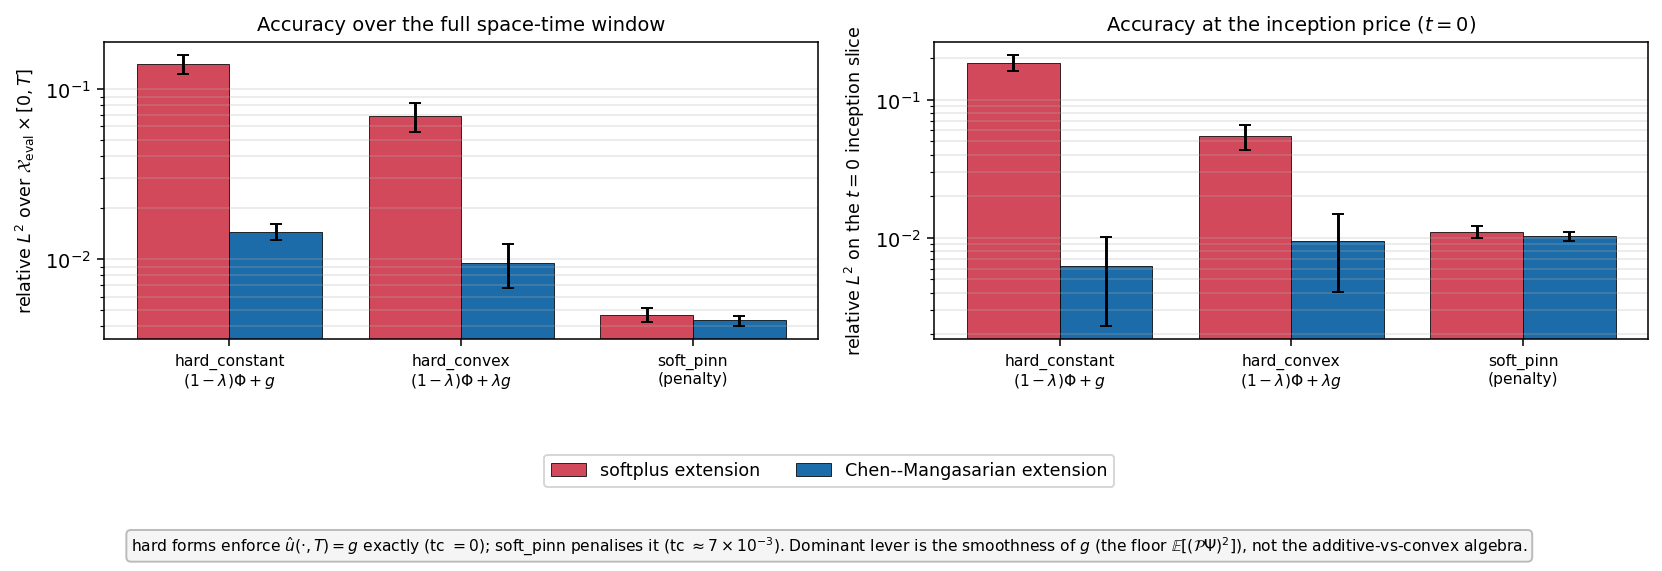
\includegraphics[width=0.98\textwidth]{figures/2026-06-12_terminal_extension_vs_mode.png}
  \caption{Accuracy per extension (colour) and form (axis), mean $\pm$ std over
    three seeds. Left: space-time window. Right: inception price.}\label{fig:h1}
\end{figure}

\begin{finding}[The extension is the dominant lever]\label{find:h1}
Holding the form fixed, replacing the softplus extension by the
Chen--Mangasarian one lowers $\relLtwo$ by a factor $9.7$ for the additive form
($1.39\times10^{-1}\to1.44\times10^{-2}$) and $7.3$ for the convex form, reaching
a factor $30$ on the inception slice. Holding the extension fixed, the
additive-to-convex change lowers $\relLtwo$ by a factor $2.0$ on the sharp
softplus datum and $1.5$ on the smooth one --- within one standard deviation for
the smooth datum. The extension controls the error by roughly an order of
magnitude, the form by a factor of two. Measured, three seeds, from
Tables~\ref{tab:main}--\ref{tab:decomp}. Hypothesis~H1 holds.
\end{finding}

\begin{observation}[Exact enforcement plus a smooth extension is competitive with the unconstrained penalty]\label{obs:h1}
The soft form has the lowest space-time error but does not satisfy the constraint
($\boundaryResidual\approx7\times10^{-3}$). With the Chen--Mangasarian extension
the hard forms close most of that gap while enforcing the datum exactly, and on
the inception slice --- the priced quantity --- the exactly-constrained additive
form ($6.22\times10^{-3}$) is more accurate than the soft form
($1.03\times10^{-2}$). Measured, three seeds, Table~\ref{tab:main}.
\end{observation}

% ===========================================================================
\section{H2 --- the error is the uncancellable operator channel}\label{sec:h2}

Hypothesis~H2 is tested directly by resolving the spatial power spectra of the two
forcing channels of \eqref{eq:channels} and of the achieved residual
$\pdeOperator\architectureOutput$, for the convex form on the sharp (softplus) and
smooth (Chen--Mangasarian) extensions (Figure~\ref{fig:h2-spectra}). The
comparison is computed at high resolution ($N=32768$ grid points) so that the
softplus operator channel --- a sub-grid curvature spike of width
$\sim1/(\beta\strike)\sim10^{-4}$ --- is represented rather than aliased.

\begin{figure}[htbp]\centering
  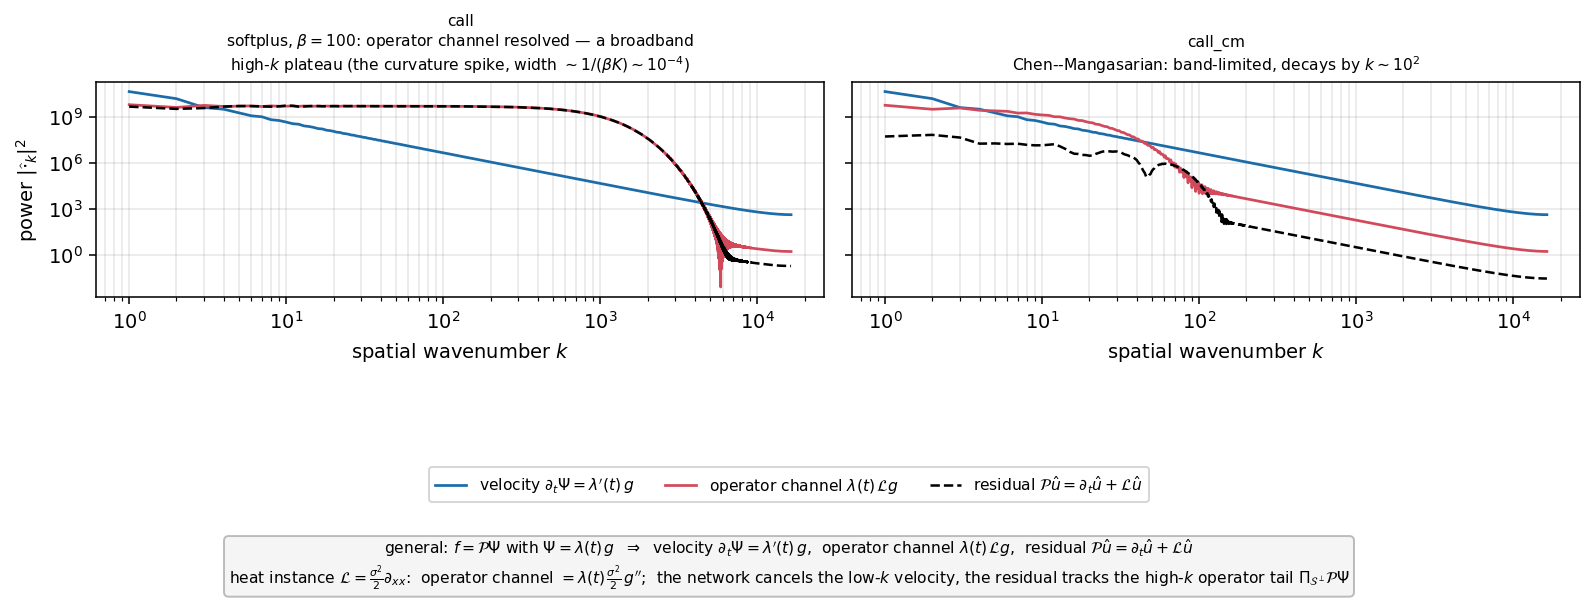
\includegraphics[width=0.98\textwidth]{figures/2026-06-12_spectral_channels_vs_residual.png}
  \caption{Channel spectra versus achieved residual (convex form, high
    resolution). Velocity channel $\interpolationCoefficient'\payoff$, operator
    channel $\interpolationCoefficient\generatorUnderlying\payoff$, and residual
    $\pdeOperator\architectureOutput$. Left: softplus. Right:
    Chen--Mangasarian.}\label{fig:h2-spectra}
\end{figure}

For the softplus extension the operator channel is the broadband white plateau of
Corollary~\ref{cor:white}, and the achieved residual coincides with it across the
band: the network cancels the low-wavenumber velocity channel but leaves the
operator spike uncancelled (Empirical finding~\ref{find:residual}). For the
Chen--Mangasarian extension the operator channel is band-limited and the residual
lies far below both channels --- it is cancellable. Figure~\ref{fig:h2-spike}
shows the softplus operator channel resolving from an aliased artefact into the
broadband plateau as the grid refines, with its band-integrated energy converging
to $\approx1.9\times10^{4}$.

\begin{figure}[htbp]\centering
  
\includegraphics[width=0.98\textwidth]{figures/2026-06-12_operator_channel_spike.png}
  \caption{Resolving the softplus operator channel. Left: the curvature spike in
    real space, which a coarse grid does not resolve. Right: its spectrum converging to
    a plateau as the grid refines.}\label{fig:h2-spike}
\end{figure}

\begin{observation}[Verdict on H2]\label{obs:h2}
The achieved error is set by the uncancellable, high-wavenumber operator channel,
not by the total floor: the sharp extension, whose operator channel is white and
uncancellable (Empirical finding~\ref{find:residual}), is the least accurate; the
smooth extension, whose operator channel is band-limited, is an order of magnitude
more accurate (Empirical finding~\ref{find:h1}). Notably the total floor is not
the predictor --- the convex Chen--Mangasarian cell has a floor of $974$, twelve
times the additive cell's $80$ (Table~\ref{tab:decomp}), yet a smaller objective
$\frakL$, because its large floor is the \emph{cancellable} velocity channel.
Hypothesis~H2 holds.
\end{observation}

% ===========================================================================
\section{H3 --- exact enforcement propagates less error}\label{sec:h3}

A Bermudan put with exercise dates $\timePoint_{1}<\dots<\timePoint_{\numExerciseDates}=\timeHorizon$
is priced by backward induction: on each inter-exercise interval the value solves
\eqref{eq:tvp}, and at each date the holder takes the smoothed maximum
$\smoothMaxCM$ of the payoff and the continuation value $\continuationValue$. The
learned induction (Section~\ref{sec:h3}) solves every interval with a hard-form
trial solution whose terminal datum is the smoothed maximum of the payoff and the
\emph{learned} value of the interval above; no analytic value is injected. Each
stage is compared against the exact chained-convolution reference of
Definition~\ref{def:exact-bermudan}; the per-date error is $\relLtwo$ on the spot
window.

Table~\ref{tab:induction} reports the two-date instance ($\numExerciseDates=2$):
the learned hard and soft forms, and the exact-continuation oracle of
Definition~\ref{def:oracle}, which supplies the analytic European continuation as
the single intermediate datum. Figures~\ref{fig:h3-prop}--\ref{fig:h3-price} show
the per-date error and the inception price.

\begin{table}[htbp]\centering
\caption{Two-date Bermudan ($\numExerciseDates=2$), mean over three seeds (seed
  standard deviation below $1\times10^{-4}$). Relative error $\relLtwo$ near maturity
  and at inception. The oracle (a single run) is supplied the exact continuation and
  learns only the remaining stage.}\label{tab:induction}
\begin{tabular}{lcc}
\toprule
form & $\relLtwo$ ($\timePoint=\timeHorizon/2$) & $\relLtwo$ (inception)\\
\midrule
hard convex (learned) & $2.15\times10^{-2}$ & $3.17\times10^{-2}$\\
soft (learned)        & $2.92\times10^{-2}$ & $4.98\times10^{-2}$\\
oracle (exact continuation) & --- & $1.2\times10^{-3}$\\
\bottomrule
\end{tabular}
\end{table}

\begin{figure}[htbp]\centering
  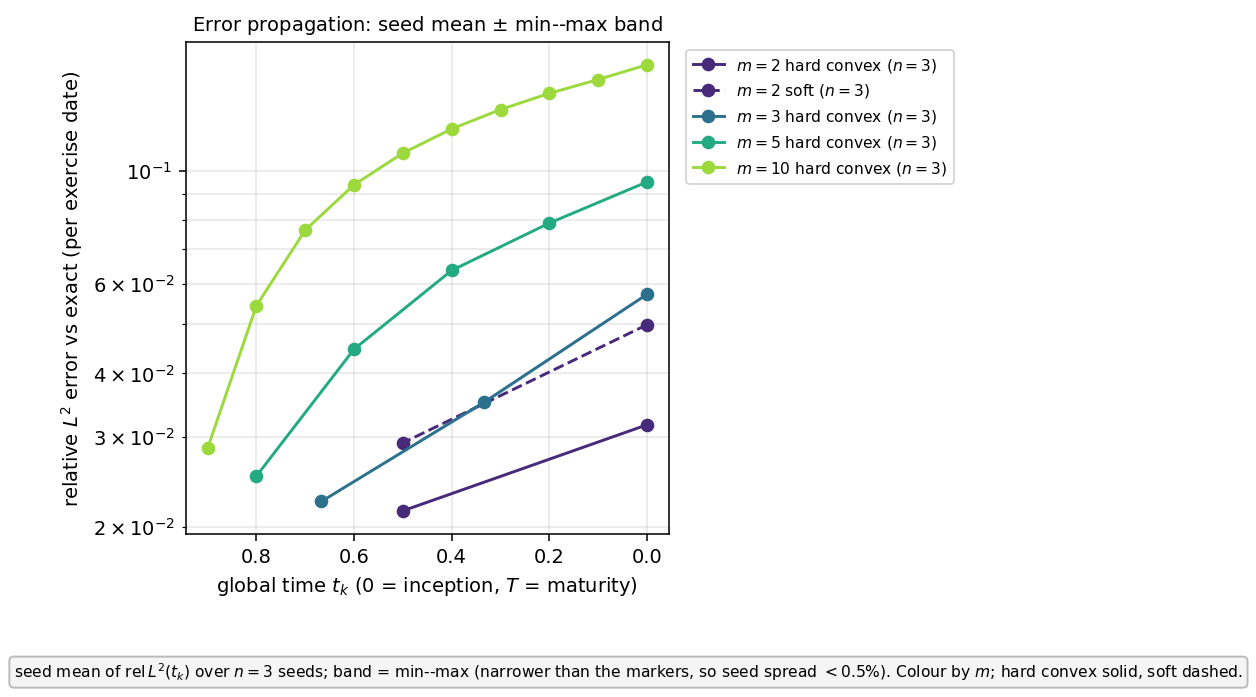
\includegraphics[width=0.82\textwidth]{figures/2026-07-06_bermudan_error_propagation_seeds.png}
  \caption{Error at each exercise date, maturity (right) to inception (left); seed
    mean over three seeds, with a min--max band narrower than the markers (seed
    spread below $0.5\%$). Colour by the number of exercise dates
    $\numExerciseDates$; hard convex solid, soft dashed. The profile is monotone
    from maturity to inception at every $\numExerciseDates$.}\label{fig:h3-prop}
\end{figure}
\begin{figure}[htbp]\centering
  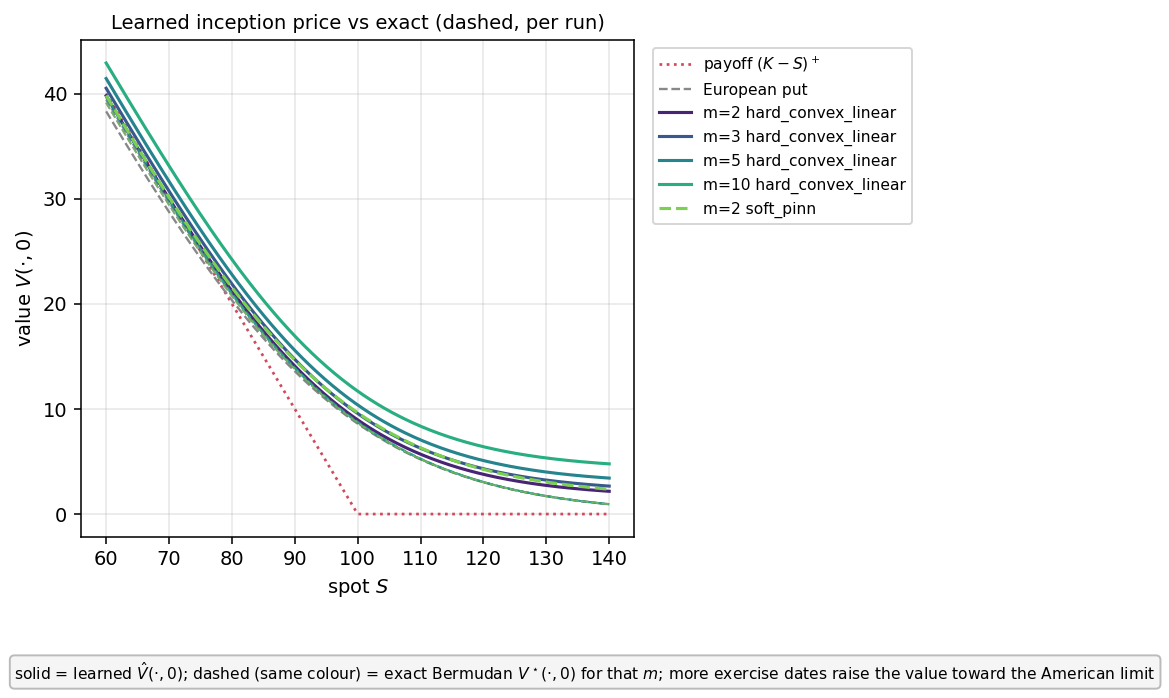
\includegraphics[width=0.82\textwidth]{figures/2026-07-06_bermudan_inception.png}
  \caption{Inception price, seed-0 chains at $\numExerciseDates\in\{2,3,5,10\}$.
    Solid: learned. Dashed (same colour): exact for that
    $\numExerciseDates$. The learned values lie above the European put (a positive
    early-exercise premium) and increase with $\numExerciseDates$.}\label{fig:h3-price}
\end{figure}

\begin{finding}[Exact enforcement propagates less error than a penalty]\label{find:h3}
Through the two-date induction the hard convex form reaches an inception error of
$3.17\times10^{-2}$ against $4.98\times10^{-2}$ for the soft form: the soft form's
per-stage terminal mismatch ($\boundaryResidual\approx7\times10^{-3}$,
Table~\ref{tab:main}) is inherited by the stage below and accumulates, whereas the
hard form carries none. The exact-continuation oracle reaches $1.2\times10^{-3}$,
so the representational limit of a single learned stage is small; the learned
chain's larger error is attributable to learning, rather than being supplied, the
continuation. Measured as the mean over three seeds (seed standard deviation below
$1\times10^{-4}$). Hypothesis~H3 holds.
\end{finding}

% ===========================================================================
\section{H4 --- accuracy is not maintained as the exercise count grows}\label{sec:h4}

Table~\ref{tab:mscaling} reports the hard convex induction at
$\numExerciseDates\in\{2,3,5,10\}$: the inception error and the error at the
first solved date (near maturity).

\begin{table}[htbp]\centering
\caption{Hard convex induction versus number of exercise dates
  $\numExerciseDates$, mean over three seeds (seed standard deviation
  $<3\times10^{-4}$ throughout). The per-date profile is monotone from maturity
  to inception, so the inception error is also the peak per-date error.}\label{tab:mscaling}
\begin{tabular}{lcc}
\toprule
$\numExerciseDates$ & $\relLtwo$ (inception) & $\relLtwo$ (first solved date)\\
\midrule
2  & $3.17\times10^{-2}$ & $2.15\times10^{-2}$ ($\timePoint=0.50$)\\
3  & $5.72\times10^{-2}$ & $2.24\times10^{-2}$ ($\timePoint=0.67$)\\
5  & $9.50\times10^{-2}$ & $2.51\times10^{-2}$ ($\timePoint=0.80$)\\
10 & $1.61\times10^{-1}$ & $2.85\times10^{-2}$ ($\timePoint=0.90$)\\
\bottomrule
\end{tabular}
\end{table}

\begin{observation}[The error grows with the number of exercise dates; H4 is refuted]\label{obs:h4}
The inception error grows monotonically with the number of exercise dates:
$3.17\times10^{-2}$, $5.72\times10^{-2}$, $9.50\times10^{-2}$, $1.61\times10^{-1}$
at $\numExerciseDates=2,3,5,10$ --- a fivefold rise from two to ten dates, with the
inception error per exercise date lying between $1.6\times10^{-2}$ and
$1.9\times10^{-2}$ at every $\numExerciseDates$ (a growth close to proportional to
$\numExerciseDates$). By contrast the error at the first solved date is essentially
independent of $\numExerciseDates$ ($2.2$--$2.9\times10^{-2}$ across the sweep,
Table~\ref{tab:mscaling}): the growth is an accumulation effect down the chain, not
a degradation of the individual solves, and the per-date profile is monotone from
maturity to inception at every $\numExerciseDates$ (Figure~\ref{fig:h3-prop}).
Section~\ref{sec:recursion} decomposes the accumulation exactly: the dominant
per-date injections are the Chen--Mangasarian smoothing bias introduced at each
exercise date and the contracted inherited error, while the interior per-stage
solve errors are one to two orders of magnitude smaller. The learned
$\numExerciseDates=10$ inception price lies visibly below its exact reference for
large spot. Measured over three seeds against the corrected exact reference (the
pre-correction reference understated the $\numExerciseDates\ge3$ errors; see
Appendix~\ref{app:repro}); the seed standard deviation is below $3\times10^{-4}$ at
every date and every $\numExerciseDates$, so the growth is a systematic effect and
not seed noise. Hypothesis~H4 is refuted.
\end{observation}

\begin{remark}[Computational cost of the learned induction grows quadratically in $\numExerciseDates$]\label{rem:cost}
Distinct from the accuracy above, the wall-clock cost of the learned induction
scales as $O(\numExerciseDates^{2})$. The terminal datum of stage $j$ is the
smoothed maximum of the payoff and the \emph{learned} continuation of stage
$j{+}1$, which is itself the trial solution embedding stage $j{+}2$, and so on;
a single residual evaluation at stage $j$ --- and its second-order automatic
differentiation --- therefore propagates through the frozen networks of every stage
above it, so the per-stage cost is proportional to the stage depth. This is measured
directly: for the $\numExerciseDates=10$ run (fixed $2\times10^{4}$ iterations per
stage) the per-stage wall-clock increases linearly with depth, from $7.1$~min at the
top interval to $37.2$~min eight intervals down --- about $4$--$4.5$~min per
additional frozen stage. Summing a linear per-stage cost over $\numExerciseDates$
stages yields the quadratic total; the measured single-seed run times are $19$, $34$
and $80$~min for $\numExerciseDates=2,3,5$. The remedy is to cache each frozen
continuation on a fixed space--time grid and interpolate, restoring an
$O(1)$-in-depth per-stage cost and an $O(\numExerciseDates)$ total; it is not needed
for the $\numExerciseDates\le10$ validation reported here.
\end{remark}

% ===========================================================================
\section{Error propagation: the recursion, its contraction, and the measured
  decomposition}\label{sec:recursion}

The growth measured in Section~\ref{sec:h4} is explained by an exact propagation
law. For the induction of Section~\ref{sec:h3} with equally spaced dates
$\timePoint_k=k\timeHorizon/\numExerciseDates$ and interval length
$\Delta=\timeHorizon/\numExerciseDates$, write $\heatSemigroup$ for the
backward-heat propagation over one interval (Gaussian convolution of variance
$\sigma^{2}\Delta$), $\continuationValue_k$ and $\continuationValue^{\star}_k$ for
the learned and exact continuation values at date $\timePoint_k$ (with
$\continuationValue_{\numExerciseDates}=\continuationValue^{\star}_{\numExerciseDates}=0$),
$\stageDatum_k=\smoothMaxCM(\payoff,\continuationValue_{k+1})$ for the learned
terminal datum of stage $k$, and
\begin{equation*}
  \stageError_k=\continuationValue_k-\continuationValue^{\star}_k,
  \qquad
  \solveError_k=\continuationValue_k-\heatSemigroup\stageDatum_k,
  \qquad
  \smoothMaxBias_{k+1}
  =\smoothMaxCM(\payoff,\continuationValue^{\star}_{k+1})
   -\max(\payoff,\continuationValue^{\star}_{k+1})
\end{equation*}
for the per-date error, the per-stage solve error, and the smoothing bias.

\begin{proposition}[Error recursion; the induction does not amplify]\label{prop:recursion}
For every $0\le k\le\numExerciseDates-1$ the pointwise identity
\begin{equation}\label{eq:recursion}
  \stageError_k
  =\solveError_k
  +\heatSemigroup\Bigl(
     \underbrace{\smoothMaxCM(\payoff,\continuationValue_{k+1})
                -\smoothMaxCM(\payoff,\continuationValue^{\star}_{k+1})}_{
                \text{inherited, }\abs{\,\cdot\,}\le\abs{\stageError_{k+1}}\ \text{pointwise}}
     +\smoothMaxBias_{k+1}\Bigr)
\end{equation}
holds, with $0<\smoothMaxBias_{k+1}\le\varepsilon/2$ pointwise. Moreover
$\heatSemigroup$ contracts both the supremum norm and the $\mathrm{L}^{2}$ norm,
and telescoping \eqref{eq:recursion} from $k=\numExerciseDates-1$ downward gives
\begin{equation}\label{eq:telescope}
  \norm{\stageError_0}_{\infty}
  \;\le\;\sum_{k=0}^{\numExerciseDates-1}\norm{\solveError_k}_{\infty}
   \;+\;\numExerciseDates\,\frac{\varepsilon}{2}.
\end{equation}
In particular the inherited error enters with operator norm at most one at every
stage: the backward induction propagates error without amplification, and growth
of the total error in $\numExerciseDates$ can arise only from the number and size
of the per-stage injections.
\end{proposition}
\begin{proof}
Adding and subtracting $\heatSemigroup\stageDatum_k$ and using
$\continuationValue^{\star}_k=\heatSemigroup\max(\payoff,\continuationValue^{\star}_{k+1})$
together with the linearity of $\heatSemigroup$ gives \eqref{eq:recursion}. The
pointwise bound on the inherited term follows from
$\partial_b\smoothMaxCM(a,b)=\tfrac12\bigl(1-\tfrac{a-b}{\sqrt{(a-b)^{2}+\varepsilon^{2}}}\bigr)\in(0,1)$,
so $\smoothMaxCM$ is $1$-Lipschitz in its second argument; the bias bound from
$\smoothMaxCM(a,b)-\max(a,b)=\tfrac12\bigl(\sqrt{(a-b)^{2}+\varepsilon^{2}}-\abs{a-b}\bigr)\in(0,\varepsilon/2]$.
$\heatSemigroup$ is convolution with the centred Gaussian density
$\varphi_{\sigma^{2}\Delta}$, and $\norm{\varphi_{\sigma^{2}\Delta}}_{\mathrm{L}^{1}}=1$,
so Young's inequality gives
$\norm{\heatSemigroup f}_{q}\le\norm{f}_{q}$ for every $q\in[1,\infty]$.
Applying the supremum norm to \eqref{eq:recursion}, using
$\heatSemigroup\smoothMaxBias\le\varepsilon/2$ (positive kernel of mass one applied
to a function bounded by $\varepsilon/2$), and iterating downward from
$\stageError_{\numExerciseDates}=0$ yields \eqref{eq:telescope}.
\end{proof}

The two constituents of Proposition~\ref{prop:recursion} --- the contraction and
the decomposition --- are each verified numerically.

\begin{finding}[The propagation is a measured contraction]\label{find:damping}
A known perturbation $\delta$ injected into one continuation of the
\emph{exact} ten-date induction and read at inception has gain
$\norm{\Delta\vFunction(\cdot,0)}/\norm{\delta}<1$ in every measured
configuration. Injecting a smoothly windowed single spatial mode at the first
intermediate date: the gain at the lowest wavenumber is $0.851$ against the heat
factor $e^{-\frac{\sigma^{2}}{2}\wavenumber^{2}\timePoint_{1}}=0.842$ (agreement
within $1.1\%$), tracks the heat prediction to within a factor two up to the
fourth mode, and floors at the probe's spectral-leakage level
($\sim10^{-2}$) beyond. Injecting a fixed smooth perturbation at each date in
turn: the inception gain decreases monotonically with the propagation distance,
from $0.851$ (injection at $\timePoint=0.1$) to $0.271$ (injection at
$\timePoint=0.9$). Measured, exact induction, no learning
(Figure~\ref{fig:damping}).
\end{finding}

\begin{finding}[The recursion decomposition, measured on the saved chains]\label{find:recursion}
Every term of \eqref{eq:recursion} was evaluated on the saved seed-0 chains at
$\numExerciseDates\in\{2,3,5,10\}$ (no training; the identity residual, including
the one-application kernel-truncation defect carried explicitly, is below
$3\times10^{-14}$ at every date, and the defect itself below $7\times10^{-6}$).
On the evaluation window, in root-mean-square value units
(Figure~\ref{fig:recursion}):
\begin{itemize}
  \item the \emph{interior} per-stage solve errors are small ---
    $\norm{\solveError_k}$ ranges from $3\times10^{-3}$ to $3\times10^{-2}$ for
    $k\le\numExerciseDates-2$ --- while the top stage, whose datum carries the
    smoothed payoff, has $\norm{\solveError_{\numExerciseDates-1}}$ between
    $0.18$ ($\numExerciseDates=10$) and $0.60$ ($\numExerciseDates=2$);
  \item the smoothing bias injects $\norm{\heatSemigroup\smoothMaxBias_{k+1}}
    \approx0.59$--$0.86$ at \emph{every} date (at the fixed $\varepsilon=2$), and
    is the dominant recurring injection --- one to two orders of magnitude larger
    than the interior solve errors;
  \item the measured inception error is $0.34$--$0.55$ of the telescoped sum
    $\sum_k(\norm{\solveError_k}+\norm{\heatSemigroup\smoothMaxBias_{k+1}})$
    across the sweep: the contraction of Empirical finding~\ref{find:damping} is
    what keeps the accumulated error at roughly half its worst-case bound.
\end{itemize}
The near-linear growth of the inception error in $\numExerciseDates$
(Observation~\ref{obs:h4}) is therefore measured to be bias-accumulation
dominated: each additional exercise date injects one further smoothing bias of
roughly constant size, damped but not removed by the subsequent propagation.
At fixed smoothing scale this contribution is structural ---
$\smoothMaxBias$ is the distance between the smoothed dynamic program the chain
actually solves and the hard-maximum reference program --- which suggests
tightening $\varepsilon$ as $\numExerciseDates$ grows; that trade-off (against
Proposition~\ref{prop:floor}, which penalises sharper data) is not measured here.
\end{finding}

\begin{figure}[htbp]\centering
  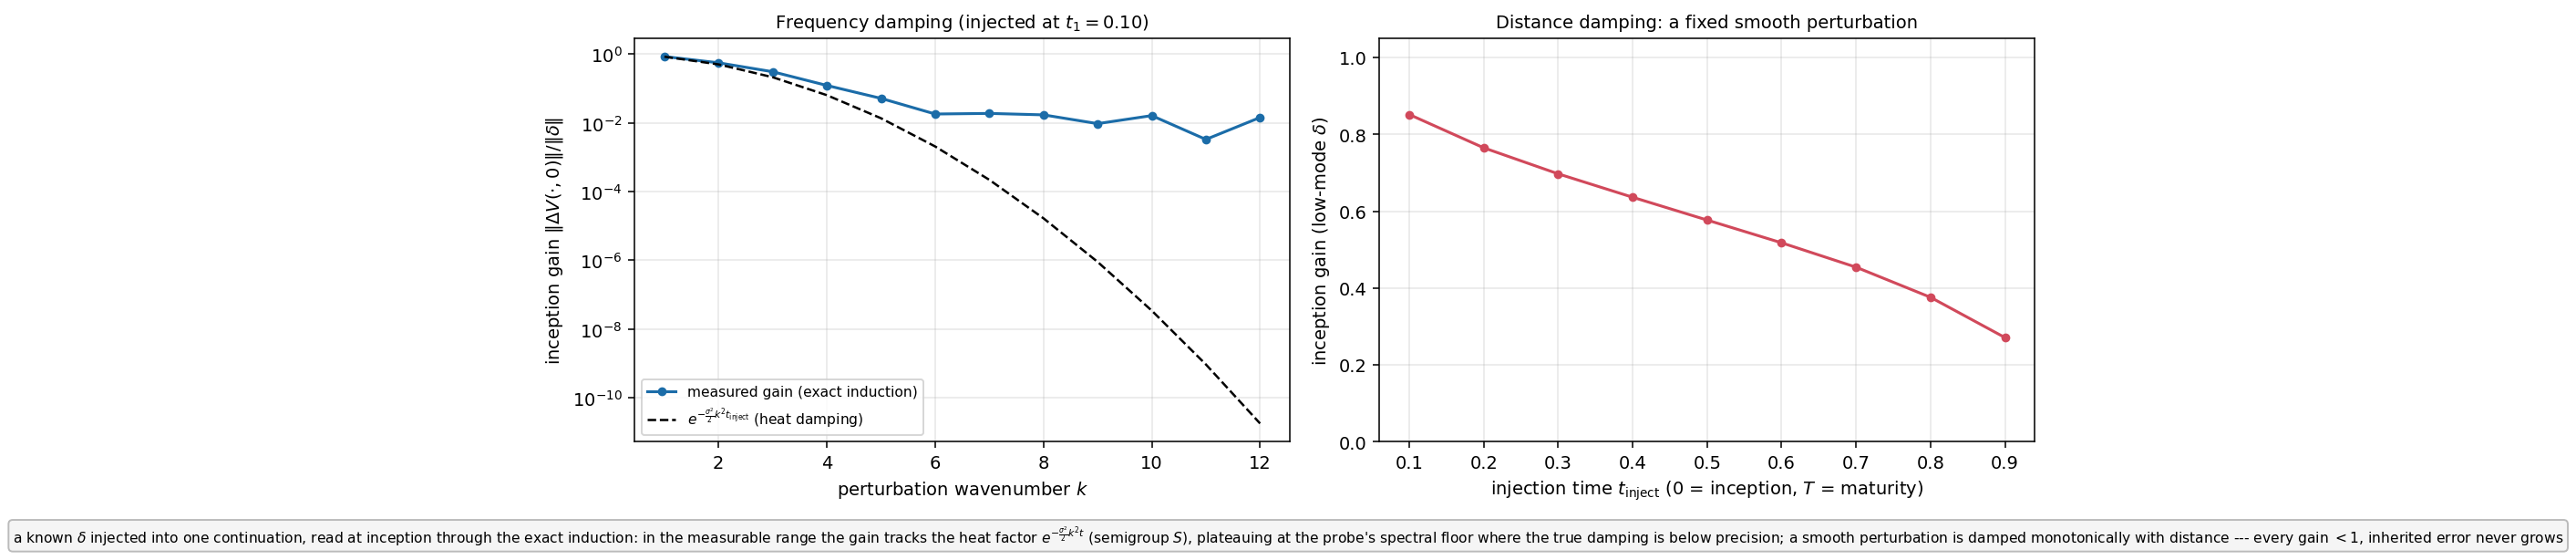
\includegraphics[width=0.98\textwidth]{figures/2026-07-05_bermudan_perturbation_propagation.png}
  \caption{The damping operator measured on the exact ten-date induction. Left:
    inception gain of a single injected mode versus its wavenumber (solid),
    against the heat factor (dashed); the gain floors at the probe's
    spectral-leakage level. Right: inception gain of a fixed smooth perturbation
    versus its injection time; monotone, all gains below one.}\label{fig:damping}
\end{figure}
\begin{figure}[htbp]\centering
  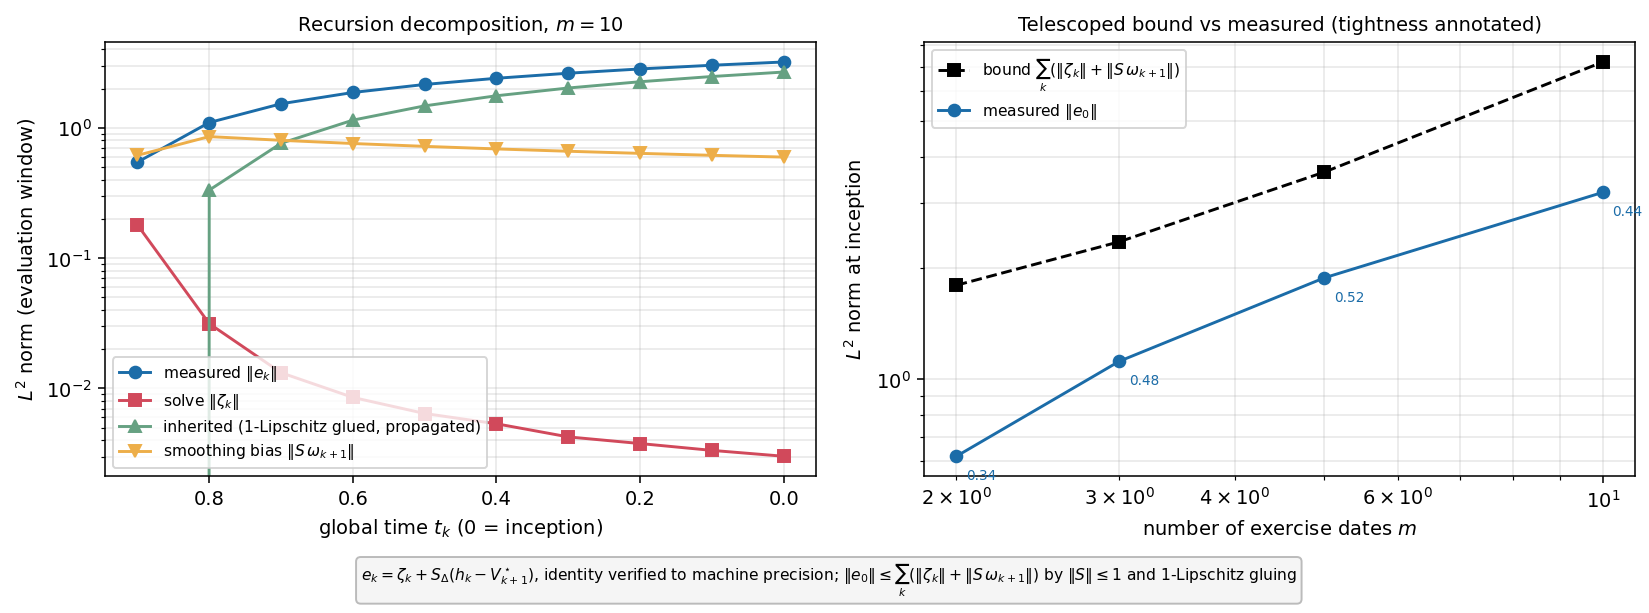
\includegraphics[width=0.98\textwidth]{figures/2026-07-06_bermudan_error_recursion_check.png}
  \caption{The recursion terms measured on the saved chains. Left: per-date
    decomposition for $\numExerciseDates=10$ --- measured error, per-stage solve
    error, inherited term, smoothing bias. Right: measured inception error
    against the telescoped bound across $\numExerciseDates$ (tightness
    annotated).}\label{fig:recursion}
\end{figure}

% ===========================================================================
\section{Mechanism: regularity, spectral decay, and the operator channel}\label{sec:mechanism}

The findings of Sections~\ref{sec:h1}--\ref{sec:h2} are explained by a chain of
Fourier estimates that is \emph{proven} (Section~\ref{sec:mech-proven}), a
closed-form model that is \emph{proven} (Section~\ref{sec:mech-toy}), measured
evidence kept \emph{separate} (Section~\ref{sec:mech-measured}), and one
\emph{conjectured} link to network trainability (Section~\ref{sec:mech-ntk}). The
Fourier convention is $\fouriertransform{\payoff}(\wavenumber)=\int_{\R}\payoff(\spacePoint)\,e^{-i\wavenumber\spacePoint}\,d\spacePoint$.

\subsection{The proven spectral laws}\label{sec:mech-proven}

\begin{definition}[Regularity index]\label{def:reg}
For a datum $\payoff$ with an isolated singularity at $\spacePoint^{\star}$ and
smooth elsewhere, the regularity index $\regularityIndex$ is the order of the
lowest derivative that is discontinuous there: $\payoff\in C^{\regularityIndex-1}$
while $\payoff^{(\regularityIndex)}$ has a jump, so $\payoff^{(\regularityIndex+1)}$
contains a Dirac mass at $\spacePoint^{\star}$.
\end{definition}

\begin{proposition}[Regularity governs spectral decay]\label{prop:decay}
Let $\payoff$ be $C^{\regularityIndex-1}$ with an isolated singularity at
$\spacePoint^{\star}$, smooth elsewhere, and
$\payoff^{(\regularityIndex+1)}=J\,\delta(\cdot-\spacePoint^{\star})+h$ with
$h\in\mathrm{L}^{1}$ near $\spacePoint^{\star}$ (a jump of size $J$ in
$\payoff^{(\regularityIndex)}$). Taking the Fourier transform on a bounded window
about $\spacePoint^{\star}$ (equivalently, of a compactly supported localisation, so
that it is a genuine function even for a non-integrable far field),
\begin{equation}\label{eq:decay}
  \abs{\fouriertransform{\payoff}(\wavenumber)}^{2}
  \sim J^{2}\,\wavenumber^{-2(\regularityIndex+1)}
  \qquad(\wavenumber\to\infty).
\end{equation}
\end{proposition}
\begin{proof}
Differentiation corresponds to multiplication by $i\wavenumber$ in the sense of
tempered distributions, so
$\fouriertransform{\payoff}(\wavenumber)=(i\wavenumber)^{-(\regularityIndex+1)}\,\fouriertransform{\payoff^{(\regularityIndex+1)}}(\wavenumber)$
for $\wavenumber\neq0$, with no boundary terms. By hypothesis
$\payoff^{(\regularityIndex+1)}=J\,\delta(\cdot-\spacePoint^{\star})+h$ with
$h\in\mathrm{L}^{1}$: the Dirac transforms to the constant
$J\,e^{-i\wavenumber\spacePoint^{\star}}$, and
$\fouriertransform{h}(\wavenumber)=o(1)$ by the Riemann--Lebesgue lemma. Hence
$\fouriertransform{\payoff}(\wavenumber)=(i\wavenumber)^{-(\regularityIndex+1)}\bigl(J\,e^{-i\wavenumber\spacePoint^{\star}}+o(1)\bigr)$,
which is \eqref{eq:decay}. The decay rate is fixed by the order of the lowest
non-integrable derivative; the smooth far field, once localised, contributes only
rapidly decreasing terms.
\end{proof}

\begin{proposition}[Elliptic amplification]\label{prop:amp}
For the generator $\generatorUnderlying$ of order $2\operatorHalfOrder$ with Fourier
symbol growing as $\abs{\wavenumber}^{2\operatorHalfOrder}$,
\begin{equation}\label{eq:amp}
  \abs{\fouriertransform{\generatorUnderlying\payoff}(\wavenumber)}^{2}
  \sim \abs{\wavenumber}^{4\operatorHalfOrder}\,\abs{\fouriertransform{\payoff}(\wavenumber)}^{2}
  \sim J^{2}\,\wavenumber^{\,4\operatorHalfOrder-2(\regularityIndex+1)} .
\end{equation}
Applying $\generatorUnderlying$ tilts the spectrum up by $\abs{\wavenumber}^{4\operatorHalfOrder}$,
moving energy towards high wavenumbers.
\end{proposition}
\begin{proof}
Multiplication by the symbol in Fourier space, then Proposition~\ref{prop:decay}.
\end{proof}

\begin{corollary}[The operator channel of a non-differentiable datum is white]\label{cor:white}
For a first-derivative discontinuity ($\regularityIndex=1$) under a second-order generator
($\operatorHalfOrder=1$) the net exponent in \eqref{eq:amp} is
$4\operatorHalfOrder-2(\regularityIndex+1)=0$: the operator channel
$\generatorUnderlying\payoff$ has a flat (white) spectrum and infinite
$\mathrm{L}^{2}$ norm. Indeed its singular part is the Dirac
$\tfrac{\sigma^{2}}{2}J\,\delta(\cdot-\spacePoint^{\star})$ (the remainder
$\tfrac{\sigma^{2}}{2}h$ lying in $\mathrm{L}^{1}$), whose transform is the constant
$\tfrac{\sigma^{2}}{2}J\,e^{-i\wavenumber\spacePoint^{\star}}$. For the call/put in
log-price the slope jump is $J=\strike$.
\end{corollary}

\begin{proposition}[Forcing-floor scaling under smoothing]\label{prop:floor}
Let $\payoff_{\smoothingScale}$ be the datum with its singularity mollified at
spatial scale $\smoothingScale$ by a kernel whose transfer function is idealised as
a low-pass cutoff at $1/\smoothingScale$, so its spectrum is essentially unchanged
for $\abs{\wavenumber}\lesssim1/\smoothingScale$ and negligible above. If
$4\operatorHalfOrder-2\regularityIndex-1>0$ the operator-channel floor is
upper-cutoff dominated and
\begin{equation}\label{eq:floor}
  \norm{\generatorUnderlying\payoff_{\smoothingScale}}^{2}
  \;\sim\;\int_{0}^{1/\smoothingScale}\wavenumber^{\,4\operatorHalfOrder-2\regularityIndex-2}\,d\wavenumber
  \;\sim\;\smoothingScale^{-(4\operatorHalfOrder-2\regularityIndex-1)} .
\end{equation}
For the first-derivative discontinuity under the heat operator ($\operatorHalfOrder=\regularityIndex=1$)
this is $\norm{\generatorUnderlying\payoff_{\smoothingScale}}^{2}\sim\smoothingScale^{-1}$:
finite once smoothed, but growing as the smoothing sharpens.
\end{proposition}
\begin{proof}
Parseval and \eqref{eq:amp} give the integrand; the cutoff at $1/\smoothingScale$
(Definition of the mollifier scale) and the assumed exponent make the integral
dominated by its upper limit, yielding \eqref{eq:floor}. A real-space check for
$\regularityIndex=1$: $\generatorUnderlying\payoff_{\smoothingScale}$ is a
regularised delta of height $\sim\smoothingScale^{-1}$ and width $\sim\smoothingScale$
carrying fixed area, so its squared norm is
$\text{height}^{2}\times\text{width}\sim\smoothingScale^{-1}$.
\end{proof}

\subsection{The analytic toy: an exactly solvable model of the mechanism}\label{sec:mech-toy}

To isolate the mechanism with no network and no optimisation, replace the free
network by its idealised spectral behaviour --- an ideal low-pass filter that
represents (hence cancels) every mode of wavenumber $\abs{\wavenumber}\le\cutoffWavenumber$
and nothing above. On the circle, with $\pdeOperator=\partial_{\timePoint}+\generatorUnderlying$
and $\terminalExtension=\interpolationCoefficient\payoff$, every mode decouples and
the residual minimisation is closed form. This is the exact realisation of the
ideal-filter oracle of Definition~\ref{def:oracle}.

\begin{proposition}[Closed-form residual and error of the ideal-filter model]\label{prop:toy}
With $\interpolationCoefficient(\timePoint)=\timePoint/\timeHorizon$ the low modes
($\abs{\wavenumber}\le\cutoffWavenumber$) are reproduced exactly, with zero residual;
for the high modes ($\abs{\wavenumber}>\cutoffWavenumber$) the free-network
coefficient vanishes, $\architectureOutput_{\wavenumber}(\timePoint)=\interpolationCoefficient(\timePoint)\,\fouriertransform{\payoff}(\wavenumber)$, and
\begin{equation}\label{eq:toy}
  \bigl(\pdeOperator\architectureOutput\bigr)_{\wavenumber}
  =\Bigl(\interpolationCoefficient'-\tfrac{\sigma^{2}}{2}\wavenumber^{2}\interpolationCoefficient\Bigr)\fouriertransform{\payoff}(\wavenumber),
  \qquad
  \bigl(\architectureOutput-\solutionField^{\star}\bigr)_{\wavenumber}
  =\Bigl(\interpolationCoefficient(\timePoint)-e^{-\frac{\sigma^{2}}{2}\wavenumber^{2}(\timeHorizon-\timePoint)}\Bigr)\fouriertransform{\payoff}(\wavenumber).
\end{equation}
The achieved residual is exactly the uncancellable projection
$\projReachablePerp\pdeOperator\terminalExtension$: the network removes the
low-wavenumber velocity channel and is left with the high-wavenumber operator
channel.
\end{proposition}
\begin{proof}
For $\abs{\wavenumber}\le\cutoffWavenumber$ the filter can set
$\architectureOutput_{\wavenumber}=\solutionField^{\star}_{\wavenumber}=\fouriertransform{\payoff}(\wavenumber)\,e^{-\frac{\sigma^{2}}{2}\wavenumber^{2}(\timeHorizon-\timePoint)}$,
which solves $\pdeOperator\solutionField^{\star}=0$ mode-wise and matches the datum
at $\timeHorizon$; the residual there is $0$. For $\abs{\wavenumber}>\cutoffWavenumber$
the network coefficient is $0$, so $\architectureOutput_{\wavenumber}=\interpolationCoefficient\fouriertransform{\payoff}(\wavenumber)$;
applying $\pdeOperator=\partial_{\timePoint}-\tfrac{\sigma^{2}}{2}\wavenumber^{2}$
mode-wise and subtracting the exact mode give \eqref{eq:toy}.
\end{proof}
The closed form \eqref{eq:toy} is additionally verified numerically to machine
precision in the reproduction script.

Figure~\ref{fig:toy-gap} sweeps the cutoff $\cutoffWavenumber$: a band-limited
datum drops exactly to zero (an exact spectral gap gives an exact solution), a
smooth datum falls exponentially, and a first-derivative discontinuity leaves the
near-flat white plateau
of Corollary~\ref{cor:white} in the residual --- yet its solution error still
decays, because the operator inverse damps the uncancelled high modes.
Figure~\ref{fig:toy-amp} shows the $\wavenumber^{4}$ amplification turning the
first-derivative discontinuity's $\wavenumber^{-4}$ datum into that plateau. Figure~\ref{fig:toy-rve} shows
that the residual and the error have different time profiles, so the residual is
not a universal predictor of the error --- the link is the $\timePoint$-dependent
operator inverse.

\begin{figure}[htbp]\centering
  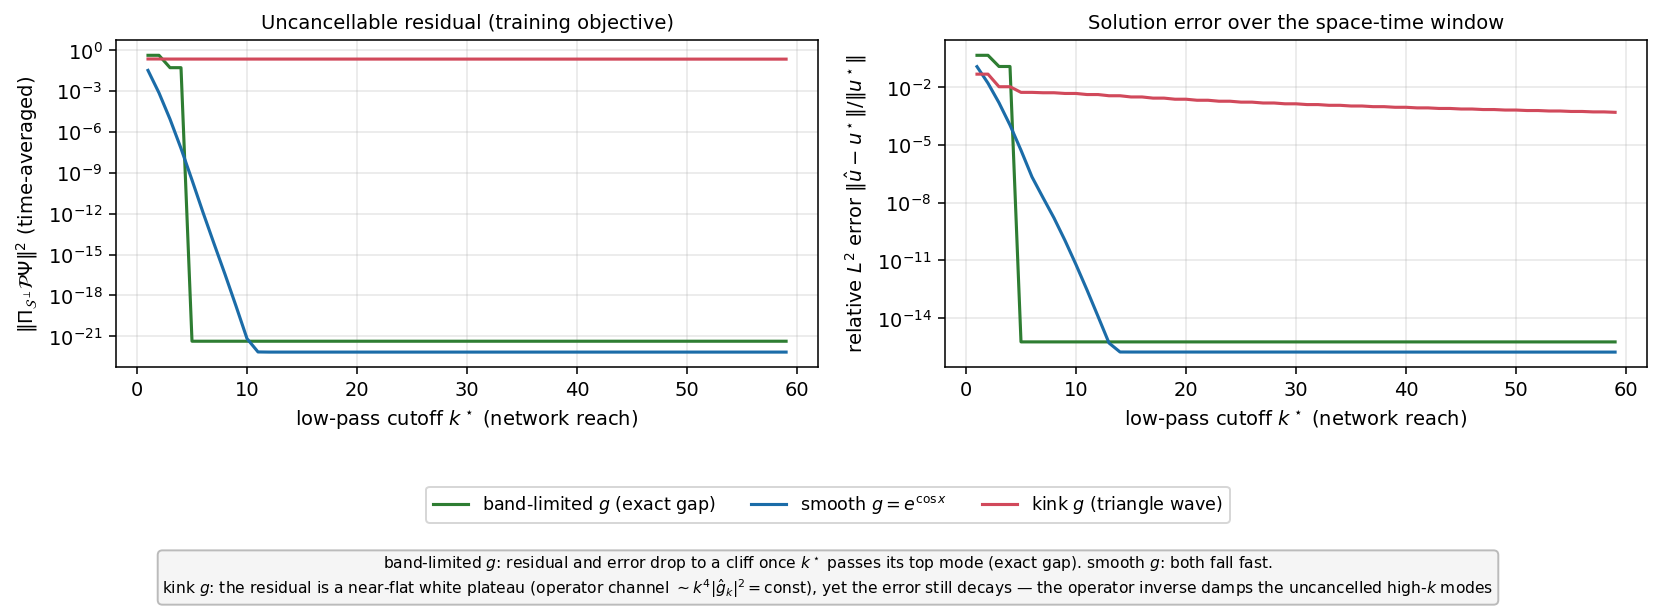
\includegraphics[width=0.98\textwidth]{figures/2026-07-03_toy_gap_vs_cutoff.png}
  \caption{Ideal-filter model. Left: the uncancellable residual versus the cutoff
    $\cutoffWavenumber$; the first-derivative discontinuity is a near-flat plateau.
    Right: the space-time
    solution error; the first-derivative discontinuity still decays. Solid curves,
    colour-coded by datum
    regularity.}\label{fig:toy-gap}
\end{figure}
\begin{figure}[htbp]\centering
  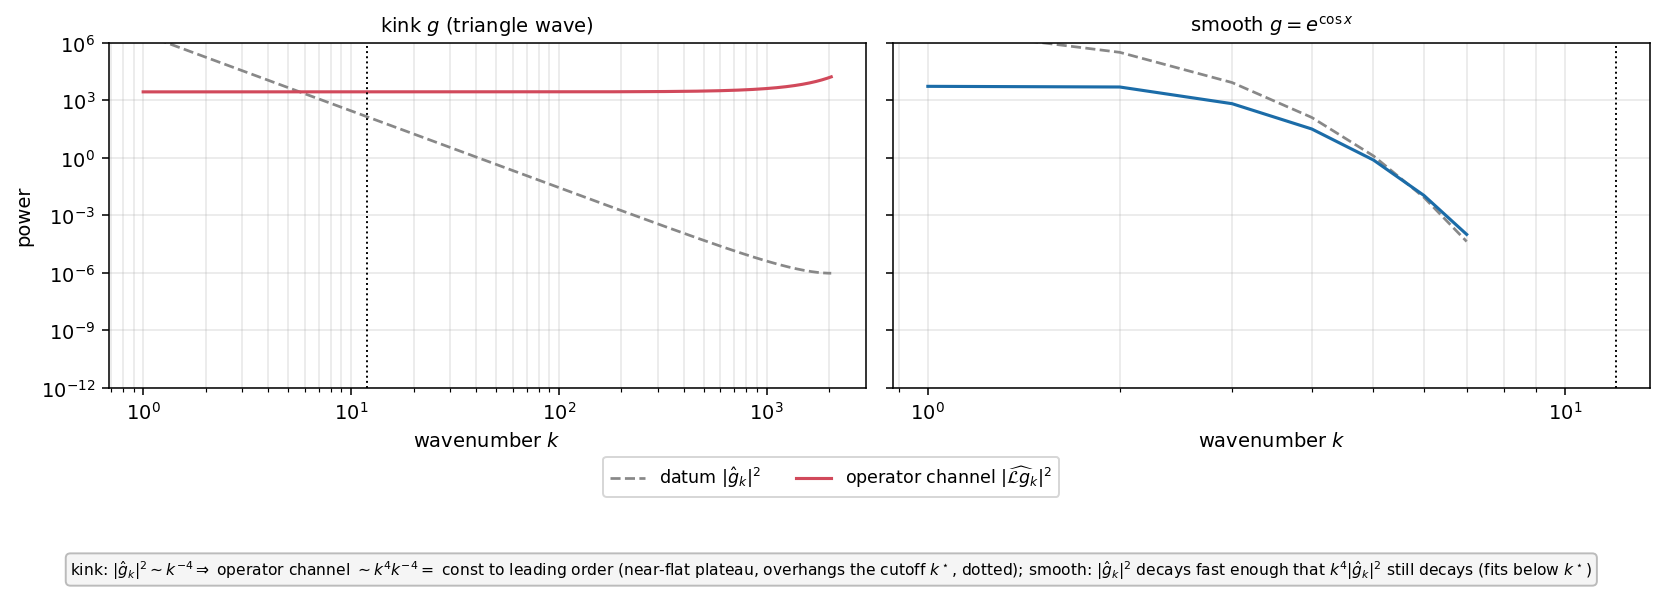
\includegraphics[width=0.98\textwidth]{figures/2026-07-03_toy_channel_amplification.png}
  \caption{The $\wavenumber^{4}$ operator amplification. Datum spectrum (dashed)
    and operator channel (solid): a first-derivative discontinuity's $\wavenumber^{-4}$ datum becomes a
    white plateau; a smooth datum stays below the cutoff (dotted).}\label{fig:toy-amp}
\end{figure}
\begin{figure}[htbp]\centering
  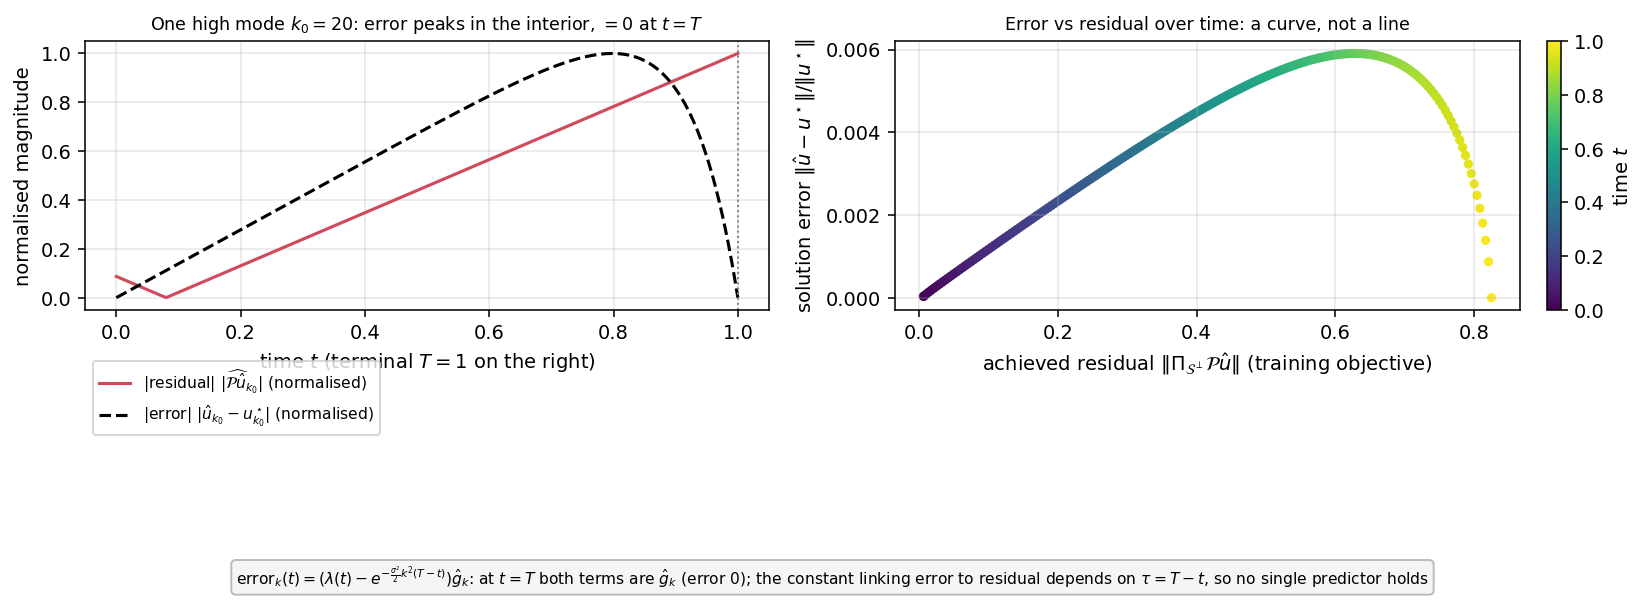
\includegraphics[width=0.98\textwidth]{figures/2026-07-03_toy_residual_vs_error.png}
  \caption{Residual is not error. Left: one high mode's residual (solid) and error
    (dashed) over time. Right: the error-versus-residual trace over time is a
    curve, not a line.}\label{fig:toy-rve}
\end{figure}

\subsection{The companion note's examples, resolved in this framework}\label{sec:mech-note}

The companion note of Charles-Albert Lehalle, \emph{Note on examples of change of
variables for gluing terminal conditions} (updated 24~May~2026;
\fp{latex_documents/reports/2026_01_29_constrained_learning_pde_lehalle_hosseinkhan/cal_notes/example_heat.tex}),
analyses the convex form of Definition~\ref{def:forms} on two data for the
backward heat equation: the two-mode sine
$\payoff=\sin(\pi\spacePoint)+c\sin(f\pi\spacePoint)$ and the Jacobi
$\vartheta_3$ series $\payoff=1+2\sum_{n\ge1}e^{-n^{2}}\cos(\pi n\spacePoint)$
--- the \texttt{sine} and \texttt{theta3} instances of the single-stage study.
(The note writes $\Psi_\theta$ for the trial field and $\Phi_\theta$ for the free
network; the report's macros, with the two glyphs interchanged, are used
throughout this subsection.) Its blending identity coincides with
\eqref{eq:residual}--\eqref{eq:channels}; the note however groups the residual as
$(1-\interpolationCoefficient)\pdeOperator\freeNetwork_{\weights}
+\interpolationCoefficient'(\payoff-\freeNetwork_{\weights})
+\interpolationCoefficient\,\generatorUnderlying\payoff$, whose middle term mixes
the $\weights$-dependent and $\weights$-independent parts, so the
$\weights$-independent floor and the channel split measured in
Table~\ref{tab:decomp} do not follow from that grouping. Likewise, the
$1/(\timeHorizon-\timePoint)$ stiffness the note reports for the linear
coefficient concerns the equation obtained after dividing the residual by
$1-\interpolationCoefficient$; the training objective of
Definition~\ref{def:learning} is the undivided residual, whose coefficients
remain bounded ($\interpolationCoefficient'=1/\timeHorizon$), and the
linear-coefficient runs of Table~\ref{tab:main} converge without difficulty.
Write $\modeDecayRate{n}=\sigma^{2}n^{2}\pi^{2}/2$ for the decay rate of the
$n$-th mode.

\begin{proposition}[Matched coefficient and the frequency-contrast leftover]\label{prop:matched}
Let $\payoff(\spacePoint)=\sin(\pi\spacePoint)+c\sin(f\pi\spacePoint)$ with
$c\neq0$ and integer $f\ge2$, let
$\interpolationCoefficient\in C^{1}([0,\timeHorizon])$ with
$\interpolationCoefficient(\timeHorizon)=1$, and let
$\terminalExtension=\interpolationCoefficient\,\payoff$ be the convex-form
extension of Definition~\ref{def:forms}. The mode-$n$ component of the
extension forcing $\pdeOperator\terminalExtension$ is
$(\interpolationCoefficient'-\modeDecayRate{n}\interpolationCoefficient)$ times
the mode, and:
\begin{enumerate}
  \item it vanishes identically if and only if
    $\interpolationCoefficient(\timePoint)=e^{\modeDecayRate{n}(\timePoint-\timeHorizon)}$;
  \item no single $\interpolationCoefficient$ annihilates the forcing of both
    modes;
  \item with the mode-$1$-matched coefficient
    $\interpolationCoefficient(\timePoint)=e^{\modeDecayRate{1}(\timePoint-\timeHorizon)}$
    the total forcing is
    \begin{equation}\label{eq:leftover}
      \pdeOperator\terminalExtension
      =-(f^{2}-1)\,\frac{\sigma^{2}\pi^{2}}{2}\,
        \interpolationCoefficient(\timePoint)\,c\,\sin(f\pi\spacePoint).
    \end{equation}
\end{enumerate}
\end{proposition}
\begin{proof}
$\generatorUnderlying\sin(n\pi\spacePoint)=-\modeDecayRate{n}\sin(n\pi\spacePoint)$,
so the mode-$n$ forcing factor is
$\interpolationCoefficient'-\modeDecayRate{n}\interpolationCoefficient$; with the
terminal value $\interpolationCoefficient(\timeHorizon)=1$ its identical
vanishing is a linear scalar ODE with the unique solution stated (i). Two modes
would force
$e^{\modeDecayRate{1}(\timePoint-\timeHorizon)}=e^{\modeDecayRate{f}(\timePoint-\timeHorizon)}$
for every $\timePoint$, impossible since $\modeDecayRate{f}=f^{2}\modeDecayRate{1}$
(ii). Substituting the matched coefficient into the mode-$f$ factor gives
$(\modeDecayRate{1}-\modeDecayRate{f})\interpolationCoefficient
=-(f^{2}-1)\tfrac{\sigma^{2}\pi^{2}}{2}\interpolationCoefficient$ (iii).
\end{proof}

The coefficient $(f^{2}-1)\sigma^{2}\pi^{2}/2$ is precisely the note's
frequency-contrast factor: it is the exact amplitude of the forcing left for the
network once the extension carries the low mode, i.e.\ a velocity--operator
mismatch on the high mode. In the ideal-filter model of
Proposition~\ref{prop:toy} this leftover is cancelled exactly when
$f\le\cutoffWavenumber$ and survives otherwise: the ``stiff, high-frequency
forcing'' of the note is the operator-channel content above the network's
cutoff --- a property of the enforcement construction, not of the problem's
posedness (the substitution $\tau=\timeHorizon-\timePoint$ turns \eqref{eq:tvp}
into a forward heat problem; the ill-posed map is the \emph{inverse} recovery of
the terminal datum from an earlier slice).

Proposition~\ref{prop:matched} is the two-mode case of a general obstruction:
a scalar coefficient can carry the exact solution precisely when the datum is
an eigenfunction, and otherwise the scalar-coefficient family has a strictly
positive forcing floor.

\begin{proposition}[Eigenfunction characterisation and positive floor]\label{prop:eigen}
Let $(\basisFunction_j)_{j\in J}$ be an orthonormal family in
$\mathrm{L}^{2}(\domain)$ with
$\generatorUnderlying\basisFunction_j=-\modeDecayRate{j}\basisFunction_j$ and
$\modeDecayRate{j}\ge0$, and let
$\payoff=\sum_{j\in J}c_j\basisFunction_j$ with
$\sum_j(1+\modeDecayRate{j}^{2})c_j^{2}<\infty$. Write
$\Sigma=\{\modeDecayRate{j}: c_j\neq0\}$ for the spectral support of the datum,
and, for $\interpolationCoefficient\in C^{1}([0,\timeHorizon])$ with
$\interpolationCoefficient(\timeHorizon)=1$, write
$\normTimeSpace{\cdot}$ for the norm of
$\mathrm{L}^{2}((0,\timeHorizon);\mathrm{L}^{2}(\domain))$, so that
\begin{equation*}
  \normTimeSpace{\pdeOperator(\interpolationCoefficient\,\payoff)}^{2}
  =\sum_{j}c_j^{2}
   \int_{0}^{\timeHorizon}
   \bigl(\interpolationCoefficient'(\timePoint)
        -\modeDecayRate{j}\interpolationCoefficient(\timePoint)\bigr)^{2}
   \,d\timePoint .
\end{equation*}
\begin{enumerate}
  \item $\pdeOperator(\interpolationCoefficient\,\payoff)=0$ for some admissible
    $\interpolationCoefficient$ if and only if $\Sigma$ is a singleton
    $\{\modeDecayRate{}\}$; in that case
    $\interpolationCoefficient(\timePoint)=e^{\modeDecayRate{}(\timePoint-\timeHorizon)}$
    and $\interpolationCoefficient\,\payoff=\solutionField^{\star}$.
  \item If $\Sigma$ contains two values $\modeDecayRate{a}<\modeDecayRate{b}$,
    carried by coefficients $c_a,c_b\neq0$, then for \emph{every} admissible
    $\interpolationCoefficient$,
    \begin{equation}\label{eq:floor-general}
      \normTimeSpace{\pdeOperator(\interpolationCoefficient\,\payoff)}
      \;\ge\;
      \min(\abs{c_a},\abs{c_b})\,
      \frac{(\modeDecayRate{b}-\modeDecayRate{a})\,\kappa_2}
           {2\bigl(1+(\modeDecayRate{b}-\modeDecayRate{a})\,\kappa_1\bigr)}
      \;>\;0,
    \end{equation}
    with $\kappa_2=\bigl(\int_0^{\timeHorizon}e^{2\modeDecayRate{a}(\timePoint-\timeHorizon)}\,d\timePoint\bigr)^{1/2}$
    and $\kappa_1=\int_0^{\timeHorizon}e^{-\modeDecayRate{a}s}\,ds$.
\end{enumerate}
\end{proposition}
The complete proof (orthonormal expansion; linear-ODE uniqueness for (i);
Duhamel representation and Young's convolution inequality for (ii)) is given
in the companion methodology document
(\fp{latex_documents/reports/2026_01_29_constrained_learning_pde_lehalle_hosseinkhan/boundary_constrained_learning_problem.tex},
Section ``Theory: the interpolation coefficient and the extension forcing''),
which aggregates the proven statements of this subsection.

The obstruction is thus attached to the \emph{rank-one form} of the extension
family $\{\interpolationCoefficient(\timePoint)\,\payoff\}$, not to the
problem: an operator-valued coefficient --- the extension
$\terminalExtension(\cdot,\timePoint)=e^{(\timeHorizon-\timePoint)\generatorUnderlying}\payoff$,
i.e.\ the exact continuation supplied to each stage by the oracle of
Definition~\ref{def:oracle} --- annihilates the forcing for every datum, and a
mode-dependent coefficient is precisely the ideal filter of
Proposition~\ref{prop:toy}. Between these extremes, \eqref{eq:floor-general}
quantifies the price of the scalar restriction by the spectral spread of the
datum, of which the note's frequency contrast
$(f^{2}-1)\sigma^{2}\pi^{2}/2=\modeDecayRate{f}-\modeDecayRate{1}$ is the
two-point case; summing the leftover over a power-law spectrum recovers the
forcing-floor scaling of Proposition~\ref{prop:floor}.

\begin{proposition}[The convex form is bias-free at the exact minimiser]\label{prop:nobias}
Let $\payoff\in C^{2}(\domain)$ be bounded with bounded
$\generatorUnderlying\payoff$ (with $\domain=\R$ or $\domain$ periodic), and let
$\solutionField^{\star}$ be the solution of \eqref{eq:tvp} in the class of
solutions bounded on $\domain\times[0,\timeHorizon]$, in which the
terminal-value problem has exactly one solution. Let
$\interpolationCoefficient\in C^{1}([0,\timeHorizon])$ satisfy
$\interpolationCoefficient(\timeHorizon)=1$,
$\interpolationCoefficient'(\timeHorizon)\neq0$, and
$\interpolationCoefficient(\timePoint)\neq1$ for $\timePoint<\timeHorizon$. Then
\begin{equation*}
  \freeNetwork^{\star}
  =\frac{\solutionField^{\star}-\interpolationCoefficient\,\payoff}
        {1-\interpolationCoefficient}
\end{equation*}
extends continuously to $\timePoint=\timeHorizon$ with value
$\payoff+\generatorUnderlying\payoff/\interpolationCoefficient'(\timeHorizon)$,
its trial field is $\architectureOutput=\solutionField^{\star}$ exactly, and the
objective of Definition~\ref{def:learning} vanishes. Among free fields
$\freeNetwork\in C^{2,1}(\domain\times[0,\timeHorizon))$ bounded on
$\domain\times[0,\timeHorizon)$ --- a class containing every network continuous
on the closed strip --- it is, for a sampler of full support, the unique zero of
the objective.
Consequently the choice of $\interpolationCoefficient$ introduces no bias at the
exact minimiser; it determines only the $\weights$-independent forcing
$\pdeOperator\terminalExtension$ that the network must cancel.
\end{proposition}
The proof (recomposition; l'H\^{o}pital at the terminal slice; terminal-value
uniqueness in the bounded class) is given in the companion methodology
document (same section as above).

\begin{lemma}[Hard enforcement excludes constant relaxation]\label{lem:relax}
No $\interpolationCoefficient\in C^{1}([0,\timeHorizon])$ with
$\interpolationCoefficient(\timeHorizon)=1$ has
$\interpolationCoefficient'/(1-\interpolationCoefficient)$ constant on
$[0,\timeHorizon)$.
\end{lemma}
The two-line integration proving this is likewise given in the methodology
document.

The note's preferred exponential blending
$b(\timePoint)=1-e^{-(\timeHorizon-\timePoint)}$ (chosen for its constant
relaxation) therefore cannot --- and does not --- satisfy the hard-enforcement
constraint: it has $b(\timeHorizon)=0$, so the trial field at maturity is the
bare network and the terminal datum must be learned, as in the soft form; the
extension weight reaches one only as $\timePoint\to-\infty$, which is the precise
content of the note's observation that its blended field ``freezes toward
$\payoff$'' in that limit.

\begin{remark}[Verdicts on the note's claims]\label{rem:note}
Three of the note's statements hold and are subsumed above: the impossibility of
matching two decay rates with one scalar coefficient
(Proposition~\ref{prop:matched}(ii)); the growth of the network's task with the
frequency contrast $(f^{2}-1)\pi^{2}/2$, which \eqref{eq:leftover} identifies as
the exact leftover forcing amplitude; and the observation that the network must
cancel a high-frequency forcing, which is the operator-channel mechanism of
Sections~\ref{sec:h2} and~\ref{sec:mech-proven}. Three require correction.
\emph{First}, ``the blended $v$ therefore differs from $u$ for $t<T$'' does not
hold for the construction itself: under
$\interpolationCoefficient(\timeHorizon)=1$ the exact minimiser reproduces
$\solutionField^{\star}$ for \emph{every} admissible coefficient
(Proposition~\ref{prop:nobias}); the discrepancy appears only through restricted
network capacity, and is then the uncancellable projection
$\projReachablePerp\pdeOperator\terminalExtension$ of
Definition~\ref{def:oracle}. Under the note's own normalisation $V(\timeHorizon,\cdot)=0$
and its blending family, the residual-zero recomposition is identically zero
(verified to $10^{-12}$), not a field freezing toward the datum; the tabulated
freeze reproduces only under the note's modal ODE, whose recomposition misses the
terminal datum entirely (its value at $\timeHorizon$ is $0$, and its deviation
from $\solutionField^{\star}$ reaches the full mode amplitude). \emph{Second},
the attribution to ``the ill-posedness of the original problem'': the
terminal-value problem \eqref{eq:tvp} is well-posed, and the note's boxed
$\vartheta_3$ solution, whose mode amplitudes grow as $\timePoint$ decreases,
satisfies $\pdeOperator\solutionField=-2\modeDecayRate{n}\solutionField\neq0$
mode-wise --- it solves the anti-diffusive equation
$\partial_{\timePoint}\solutionField-\generatorUnderlying\solutionField=0$
instead. With the operator-consistent decaying amplitudes the nome
$e^{-1-\modeDecayRate{1}(\timeHorizon-\timePoint)}$ remains below one for every
horizon, so the claimed divergence at
$\timeHorizon-\timePoint\ge2/(\sigma^{2}\pi^{2})$, and the concluding statement
that no bounded coefficient recovers the exact solution, do not survive the sign
correction (the recovery is Proposition~\ref{prop:nobias}). \emph{Third},
several algebraic defects: the sign of $b'$ and of $b'/(1-b)$ for the
exponential family differs between the note's two sections; the
generic-exponential paragraph omits the operator-channel forcing from its modal
ODE; and the boxed ``Choice~1'' $\vartheta_3$ formula solves none of the four
sign/normalisation readings of its own modal equation (residuals of order one).
Every verdict above is verified numerically to the stated precision by the
reproduction script (Appendix~\ref{app:repro}).
\end{remark}

\begin{finding}[The note's two data corroborate the mechanism]\label{find:note}
Measured on the single-stage study (three seeds, the architecture and budget of
Table~\ref{tab:main}; $\sigma=1$, $\timeHorizon=0.1$): the $\vartheta_3$ datum
--- analytic, coefficients $2e^{-n^{2}}$, hence super-exponential spectral decay
by Proposition~\ref{prop:decay} --- reaches
$\relLtwo=1.47\times10^{-3}\pm1.3\times10^{-4}$ (additive form, linear
coefficient), while the two-mode sine at $(c,f)=(0.5,4)$ reaches
$6.8\times10^{-2}$ to $1.1\times10^{-1}$ across the hard forms: a factor
$\approx50$ between the two data at identical budget, set by the datum's
frequency content. The mode-$1$-matched exponential coefficient (the note's
ideal rate $\modeDecayRate{1}$, the study's \texttt{exp} variant) lowers the
convex-form error against the linear coefficient on both data: from
$6.7\times10^{-3}\pm2.6\times10^{-4}$ to $1.9\times10^{-3}\pm2.1\times10^{-4}$
on $\vartheta_3$ (a factor $3.5$, far beyond the seed spread), and from
$1.06\times10^{-1}\pm7.4\times10^{-3}$ to $7.3\times10^{-2}\pm2.3\times10^{-2}$
on the sine (consistent within $1.5$ standard deviations) --- the measured trace
of annihilating the dominant mode's forcing
(Proposition~\ref{prop:matched}(i)).
\end{finding}

\begin{figure}[htbp]\centering
  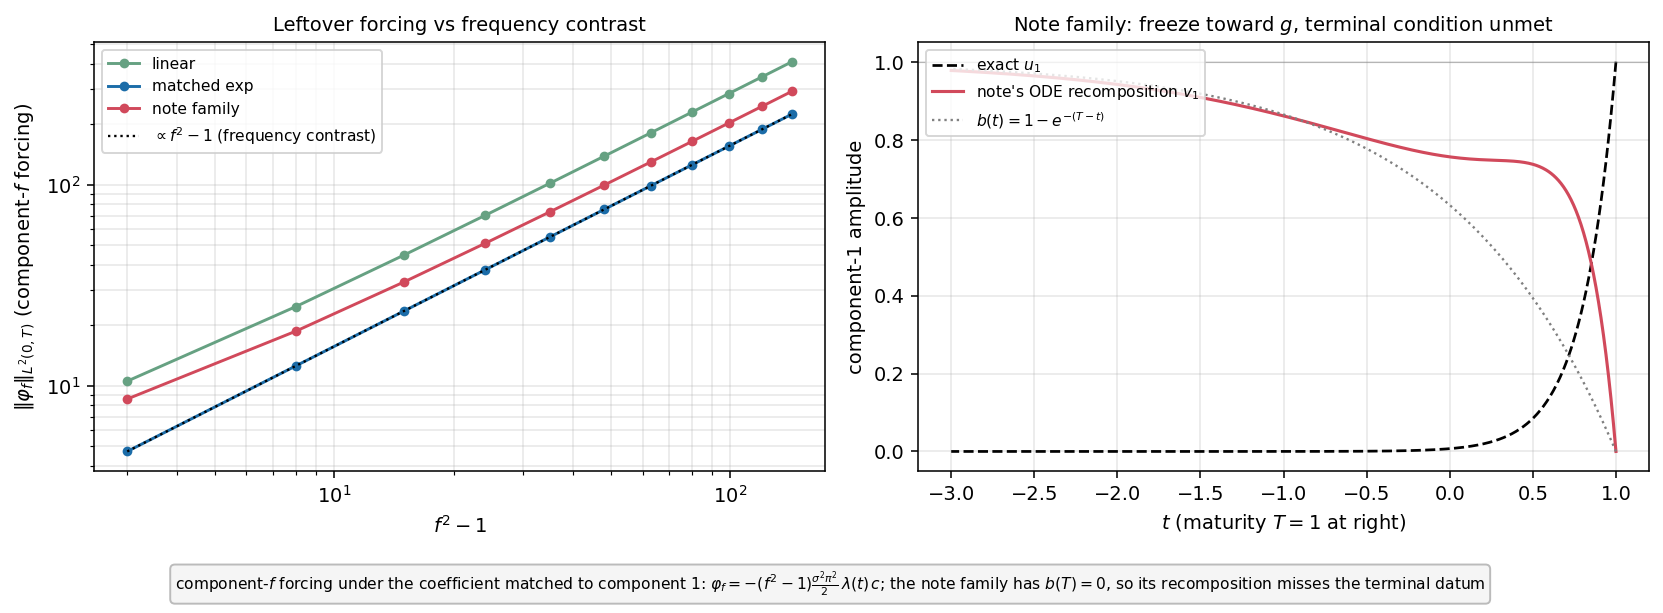
\includegraphics[width=0.98\textwidth]{figures/2026-07-08_reference_note_analysis.png}
  \caption{The note's examples verified. Left: $\mathrm{L}^{2}$-in-time norm of
    the mode-$f$ forcing against $f^{2}-1$ for the linear, matched-exponential,
    and note-family coefficients; the matched coefficient follows the
    frequency-contrast growth of \eqref{eq:leftover} exactly. Right: mode-$1$
    trajectories under the note's family and its own modal ODE --- the
    recomposition misses the terminal datum ($v(\timeHorizon)=0$) and freezes
    toward the datum only as $\timePoint\to-\infty$.}\label{fig:note}
\end{figure}

\begin{finding}[Variational check of the scalar-coefficient floor]\label{find:floor-variational}
The forcing functional of Proposition~\ref{prop:eigen} is quadratic in the
coefficient, so its minimiser subject to
$\interpolationCoefficient(\timeHorizon)=1$ is computed \emph{exactly} (one
banded linear system on a $4001$-point time grid; no training), giving the
true optimum of the whole scalar family. Measured
(Figure~\ref{fig:floor-variational}): for a single-mode datum the optimal
floor is $4.6\times10^{-13}$ and the minimiser coincides with the matched
exponential to $4.7\times10^{-8}$ (part~(i)); across the two-mode sweep
$f=2,\dots,12$ the proven lower bound \eqref{eq:floor-general} lies below the
optimum, which lies below the matched-coefficient reference, at every gap
(the bound is conservative --- optimum-to-bound ratio $5.3$ at $f=2$ rising
to $37$ at $f=12$). On the study's instances ($\timeHorizon=0.1$): for the
$\vartheta_3$ datum the matched exponential is variationally optimal among
scalar coefficients (optimum $0.1363$ against $0.1367$; the linear coefficient
lies a factor $13$ above), explaining the measured factor $3.5$ of Empirical
finding~\ref{find:note}; for the two-mode sine the optimal floor ($4.45$)
lies \emph{below} the linear ($6.37$) and matched-exponential ($9.33$)
floors, yet the measured accuracy of Empirical finding~\ref{find:note}
orders the two fixed coefficients the other way --- consistent with the
verdict on H2: the total floor is not the error predictor; the matched
coefficient concentrates its (larger) floor on the single mode $f=4$, which
lies within the network's reach and is cancelled.
\end{finding}

\begin{figure}[htbp]\centering
  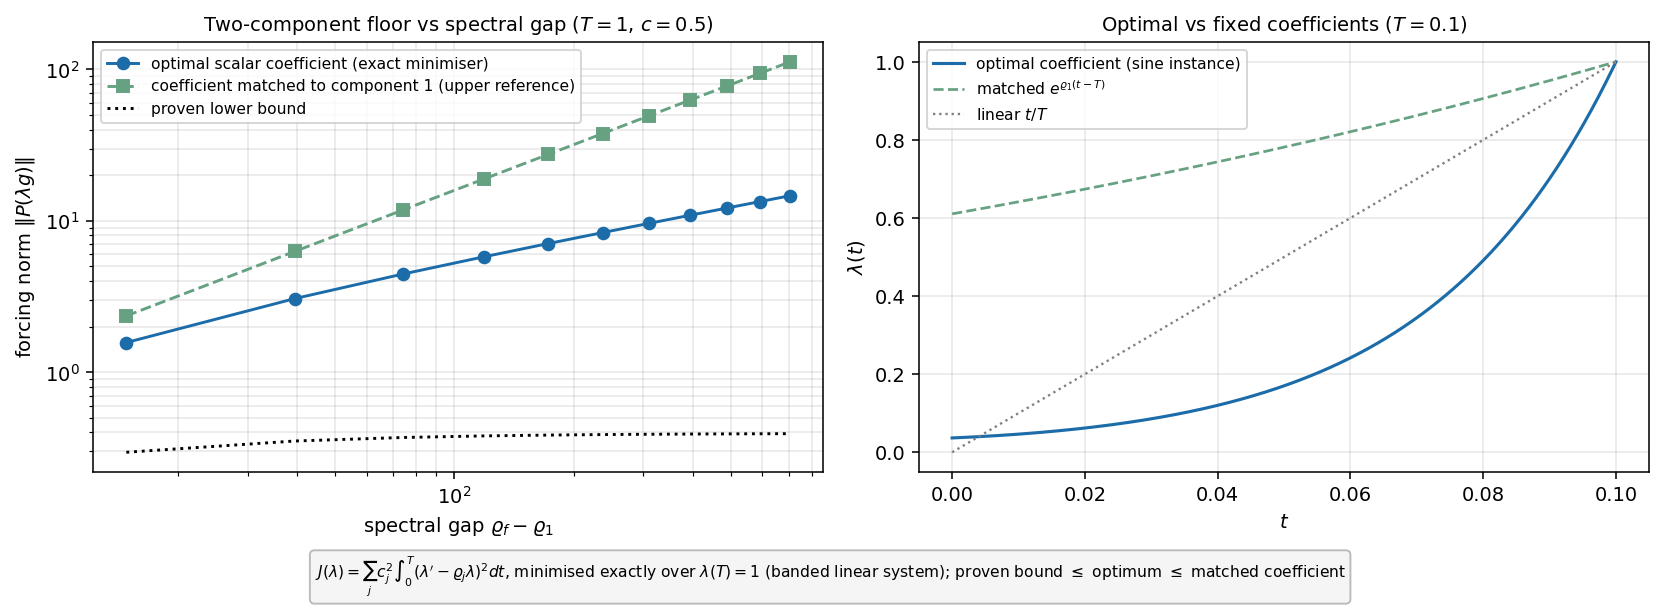
\includegraphics[width=0.98\textwidth]{figures/2026-07-09_optimal_coefficient_floor.png}
  \caption{Variational check of the scalar-coefficient floor. Left: proven
    lower bound, exact optimum, and matched-coefficient reference against the
    spectral gap (two-mode datum, $\timeHorizon=1$). Right: the optimal
    coefficient against the matched exponential and the linear coefficient on
    the sine instance ($\timeHorizon=0.1$).}\label{fig:floor-variational}
\end{figure}

\subsection{Measured confirmation (kept separate from the proofs)}\label{sec:mech-measured}

\begin{finding}[The operator channel is the achieved residual]\label{find:residual}
On the high-resolution spectra of Section~\ref{sec:h2} the achieved residual of
the sharp (softplus) extension coincides with its operator channel across the
whole band --- their band-integrated energies agree to two significant figures
($6.33\times10^{3}$ against $6.34\times10^{3}$) --- while for the smooth
(Chen--Mangasarian) extension the residual lies far below the forcing
($8.85\times10^{-1}$). Measured, one seed, from the spectra of
Figure~\ref{fig:h2-spectra}.
\end{finding}

\begin{finding}[The floor ratio matches the effective-cutoff ratio]\label{find:floor}
The measured operator-channel floor of the additive form is $7.2\times10^{3}$ for
the softplus extension against $9.1\times10^{1}$ for the Chen--Mangasarian one, a
ratio $\approx79$ (Table~\ref{tab:decomp}), consistent with
Proposition~\ref{prop:floor}: at fixed payoff and operator the floor ratio is, to
leading order, the ratio of effective smoothing cutoffs. Measured, mean over three
seeds.
\end{finding}

\subsection{The conjectured trainability link}\label{sec:mech-ntk}

\begin{remark}[Spectral bias, conjectured]\label{rem:ntk}
The step from ``white forcing'' to ``error-dominating'' rests on identifying the
network-reachable subspace $\reachableSet$ with the low-wavenumber band. Under the
neural-tangent-kernel approximation of training, gradient descent fills
$\reachableSet$ in decreasing kernel-eigenvalue order, which on a bounded domain
corresponds to increasing wavenumber, so within a finite budget
$\reachableSet\approx\{\text{low }\wavenumber\}$ and
$\reachableSetPerp\approx\{\text{high }\wavenumber\}$. This identification is
corroborated by the measured spectra of Section~\ref{sec:h2} but is not proven
here; the ideal-filter model of Proposition~\ref{prop:toy} assumes it in its
sharpest (hard-cutoff) form.
\end{remark}

% ===========================================================================
\section{Conclusion}\label{sec:conclusion}

Four hypotheses received verdicts. The regularity of the terminal extension
controls the achieved error by an order of magnitude, the trial-solution algebra
by a factor of two (H1, held); the achieved error is the uncancellable
high-wavenumber operator channel, not the total floor (H2, held --- reinforced by
the variational floor check of Empirical finding~\ref{find:floor-variational});
exact terminal enforcement propagates less error through a Bermudan backward
induction than a soft penalty (H3, held); but accuracy is not maintained as the
number of exercise dates grows (H4, refuted at ten dates). The propagation itself
is governed by a proven recursion: the induction contracts inherited error
(Proposition~\ref{prop:recursion}, measured in Empirical
findings~\ref{find:damping}--\ref{find:recursion}), and the near-linear growth in
the number of exercise dates is measured to be dominated by the smoothing bias
injected at each date, not by amplification. The single-solve mechanism is proven
as a chain of Fourier estimates, a closed-form filter model, and an eigenfunction
characterisation of the scalar-coefficient family (Proposition~\ref{prop:eigen})
that resolves and generalises the companion note's two examples
(Section~\ref{sec:mech-note}); the one step from spectral content to network
trainability remains conjectural (Remark~\ref{rem:ntk}). The measured results
rest on three seeds for the induction (the error growth is systematic, seed
standard deviation below $3\times10^{-4}$), a single architecture, and four data
(the smoothed call, the Bermudan chain, and the note's sine and $\vartheta_3$
instances); the scaling of the smoothing parameter with the number of exercise
dates, and the neural-tangent-kernel identification of the reachable subspace,
are the open directions.

% ===========================================================================
\appendix
\section{Spot Greeks}\label{app:greeks}

In the log-price coordinate $\spacePoint=\ln\spot$ the spot sensitivities of a
value field $\vFunction$ are $\Delta=\partial_{\spot}\vFunction=e^{-\spacePoint}\partial_{\spacePoint}\vFunction$
and $\Gamma=\partial^{2}_{\spot\spot}\vFunction=e^{-2\spacePoint}(\partial_{\spacePoint\spacePoint}\vFunction-\partial_{\spacePoint}\vFunction)$,
compared against the reference Greeks by relative $\mathrm{L}^{2}$ error over the
evaluation window. On the smoothed European instances all four forms of
Definition~\ref{def:forms} reproduce $\Delta$ and $\Gamma$ within the evaluation
window; the second derivative $\Gamma$ is the hardest, with its largest error at
the money, consistent with the operator channel of Section~\ref{sec:mechanism}
being a curvature at the strike.

\section{The exact multi-stage Bermudan reference}\label{app:exact}

\begin{definition}[Exact Bermudan value]\label{def:exact-bermudan}
For exercise dates $\timePoint_{1}<\dots<\timePoint_{\numExerciseDates}=\timeHorizon$
the exact value solves the dynamic program with $\vFunction(\timeHorizon,\cdot)=\payoff$,
$\continuationValue(\timePoint_{j},\cdot)=e^{(\timePoint_{j+1}-\timePoint_{j})\generatorUnderlying}\vFunction(\timePoint_{j+1},\cdot)$,
$\vFunction(\timePoint_{j},\cdot)=\max(\payoff,\continuationValue(\timePoint_{j},\cdot))$.
Between exercise dates the propagation is the exact heat semigroup, i.e.\ Gaussian
convolution (one step per interval, no time discretisation), and the maximum is
taken exactly. This is the machine-precision target of Definition~\ref{def:reference};
its defining properties (the continuation at the last intermediate date equals the
European value, the value at maturity is the payoff, the value dominates the
European value, it is monotone in $\numExerciseDates$, and the dynamic-programming
tower property $\vFunction(\timePoint_1,\cdot)=\max(\payoff,\heatSemigroup\vFunction(\timePoint_2,\cdot))$
holds on a four-date chain) are verified in the test
suite.
\end{definition}

\section{Reproduction}\label{app:repro}

Every figure and number traces to a named script in the repository
\texttt{constrained\_learning\_option\_pricing} and a run directory under
\texttt{data/}. Figure scripts derive their data folder from their own filename.

The scripts below are located under
\fp{experiments/python_scripts/exp_ansatz_forms_heat/} unless a fuller path is
given.
\begin{itemize}
  \item \textbf{Comprehensive results and H1} (Tables~\ref{tab:main}--\ref{tab:decomp},
    Figure~\ref{fig:h1}): trainer \fp{ablation_ansatz_forms.py}; cross-seed
    aggregation \fp{ansatz_forms_cross_seed_summary.py}; figure
    \fp{terminal_extension_vs_mode_comparison.py}. Runs
    \fp{data/ablation_ansatz_forms/*_call*_iters20000_seed{0,1,2}} and the
    \texttt{call\_cm} twin.
  \item \textbf{H2 spectra} (Figures~\ref{fig:h2-spectra}--\ref{fig:h2-spike},
    Empirical findings~\ref{find:residual}--\ref{find:floor}):
    \fp{spectral_gap_analysis.py} (high-resolution channel split and spike
    resolution), reading the trained \texttt{seed0} call / call\_cm models.
  \item \textbf{Mechanism toy} (Proposition~\ref{prop:toy},
    Figures~\ref{fig:toy-gap}--\ref{fig:toy-rve}):
    \fp{spectral_toy_operator_channel.py} (torch-free; prints the numerical
    self-check of the closed-form residual, including an operator-channel probe).
  \item \textbf{H3/H4 induction} (Tables~\ref{tab:induction}--\ref{tab:mscaling},
    Figures~\ref{fig:h3-prop}--\ref{fig:h3-price}): driver
    \fp{bermudan_backward_induction.py}; cross-run and seed-aggregated figures
    \fp{bermudan_induction_comparison.py} (\texttt{--aggregate-seeds}); exact
    reference \fp{learning_option_pricing/pde/heat_references.py}
    (\texttt{bermudan\_put\_value\_exact}). Runs
    \fp{data/bermudan_backward_induction/2026-07-04-*_m{2,3,5,10}_*_seed{0,1,2}}
    and the \texttt{soft\_pinn} twin, trained on Jean~Zay (\texttt{akz@v100}).
    \emph{Reference correction:} the original reference implementation carried a
    late-binding closure defect that propagated every intermediate stage to
    $\timePoint_1$ instead of $\timePoint_k$, understating the exact value's
    diffusion for three or more dates; it was detected by the truncation-defect
    self-check of the recursion verification, fixed (commit \texttt{03e8fc1},
    regression tests \fp{test/pde/test_heat_references.py}), and every run above
    was revalidated against the corrected reference
    (\texttt{--revalidate}; the trained models are unaffected --- the training
    objective is reference-free). The two-date results were unchanged; the
    $\numExerciseDates\ge3$ errors increased.
  \item \textbf{Error recursion} (Proposition~\ref{prop:recursion},
    Empirical findings~\ref{find:damping}--\ref{find:recursion},
    Figures~\ref{fig:damping}--\ref{fig:recursion}): damping measurement
    \fp{bermudan_perturbation_propagation.py} (exact induction, gains persisted
    to \texttt{gains.yaml}); identity decomposition
    \fp{bermudan_error_recursion_check.py} (rebuilds the saved chains, verifies
    the identity to $3\times10^{-14}$, writes \texttt{recursion\_check.yaml});
    post-processing executed on Jean~Zay \texttt{prepost}.
  \item \textbf{Companion-note examples} (Section~\ref{sec:mech-note},
    Empirical findings~\ref{find:note} and~\ref{find:floor-variational},
    Figures~\ref{fig:note} and~\ref{fig:floor-variational}):
    \fp{reference_note_two_mode_theta3_analysis.py} (torch-free; closed forms
    and independent ODE integration; checks the frequency-contrast leftover to
    $10^{-14}$, the bias-freeness to $10^{-14}$, the note-family recompositions
    to $10^{-12}$, the $\vartheta_3$ sign, and the boxed Choice-1 formula
    against all four readings of its modal equation; writes
    \texttt{analysis\_summary.yaml}); variational floor check
    \fp{optimal_coefficient_floor.py} (exact quadratic minimisation over the
    scalar family, banded linear system; writes \texttt{optimal\_floor.yaml});
    both executed on Jean~Zay \texttt{prepost}. Measured accuracies from the
    \texttt{sine} / \texttt{theta3} runs
    \fp{data/ablation_ansatz_forms/*_{sine,theta3}_iters20000_seed{0,1,2}}.
    Proofs of the propositions of Section~\ref{sec:mech-note} are aggregated
    in the companion methodology document
    \fp{boundary_constrained_learning_problem.tex} (same repository as the
    companion note).
\end{itemize}

\end{document}
